% !TEX encoding = UTF-8 Unicode

\documentclass[12pt,a4j,titlepage]{ltjsarticle}
\usepackage{sty/semi}
\usepackage{titlesec}


% \title{}
% \author{}
% \date{}

\begin{document}

\begin{titlepage}
  \begin{center}
  
    \vspace*{20truept}
    
    {\LARGE 2022年度 卒業論文}
    
    \vspace*{75truept}
    
    {\Huge 初学者向けネットワーク通信の学習を} %論文タイトル

    \vspace{10truept}

    {\Huge 支援するシミュレータWeb教材 } %論文タイトル 長い場合 改行1

    \vspace{10truept}

    {\Huge } %論文タイトル 改行2

    \vspace{85truept}
    
    {\LARGE 指導教員 須田 宇宙 准教授}
    
    \vspace{60truept}
    
    {\LARGE 千葉工業大学 情報ネットワーク学科}
    
    \vspace{15truept}
    
    {\LARGE 須田研究室}
    
    \vspace{70truept}
    
    {\LARGE 1932047 氏名 小松崎 嵩史 } % 氏名は消さない 学生番号 氏名 名前

    \vspace{70truept}
    
  \end{center}
  \begin{flushright}

    {\LARGE 提出日 2023年1月17日}
  
  \end{flushright}
\end{titlepage}
\setcounter{page}{0}\pagenumbering{roman}\pagestyle{plain}
\tableofcontents
% 表目次
\listoftables
% 図目次
\listoffigures

\clearpage
\setcounter{page}{0}\pagenumbering{arabic}
\section{緒言}%<1章>

%背景
DX(Digital Transformation)の実現に向けて,IT人材の確保・育成は一番大きな課題となっている.
IT人材の確保・育成を促進するため,2020年より小学校プログラミング教育から始まる情報教育の推進が図られている.
2022年より,高等学校においても新しい学習指導要領が改訂され,「情報Ⅰ」が共通必履修科目となっている.
また,大学入学共通テストにおいて2025年1月より,「情報Ⅰ」が出題範囲の「情報」が新教科として出題される予定となっている.

%問題点
情報教育の学習内容において,ネットワークの学習はプログラミングに比べて,講義形式の授業が多くなる.
しかし,講義形式の授業では初学者がネットワーク通信の階層の動きや違いを,紙面の文字や図だけで理解することが難しいため問題となる.
実習形式の授業が難しい理由として,学習指導要領でプログラミングを実習形式の授業で指導することが勧められている点や,ネットワークの実習に,通信機器,仮想環境などの準備が難しいなどの理由が考えられる.

%目的
これらの問題に対して,生徒や学生に配布されるタブレットや,小型のPCで利用できるWeb教材をネットワーク通信を学習する講義形式の授業の補助に利用することで,問題点の改善に繋がると考えた.
そこで,本研究では上記のWeb教材を作成することを目的とする.
\clearpage

\section{DXについて}%<2章>
本章では,日本におけるDXの現状について説明する.
\subsection{概要}
DXとは,Digital Transformationの略称である.
企業がグローバル環境の激しい変化に対応し,データとデジタル技術を活用して,顧客や社会のニーズを基に,製品やサービス,ビジネスモデルを変革することである.
また,業務そのものだけでなく,組織,企業文化・風土を変革し,持続的な企業価値の向上を図ることである\cite{dx_gaiyou}. 


\subsection{DX推進の課題}
国内外の企業に向けた調査内にある,デジタル化を進める上での課題や障壁の日本企業(n=1296)の解答を抜き出したグラフを図\ref{fig:dx}に示す\cite{dx_kadai}.
デジタル化を進める上での課題や障壁として,人材不足が67.6\%と最も多く,次にデジタル技術の知識・リテラシー不足が44.8\%となっている.
IT人材の不足の解決には,社内人材の育成やアウトソーシングといった方法が考えられるが,持続的な企業価値の向上を図るためには,将来にわたって情報教育の推進が必要だと考えられる.
\\
\begin{figure}[h]
\centering
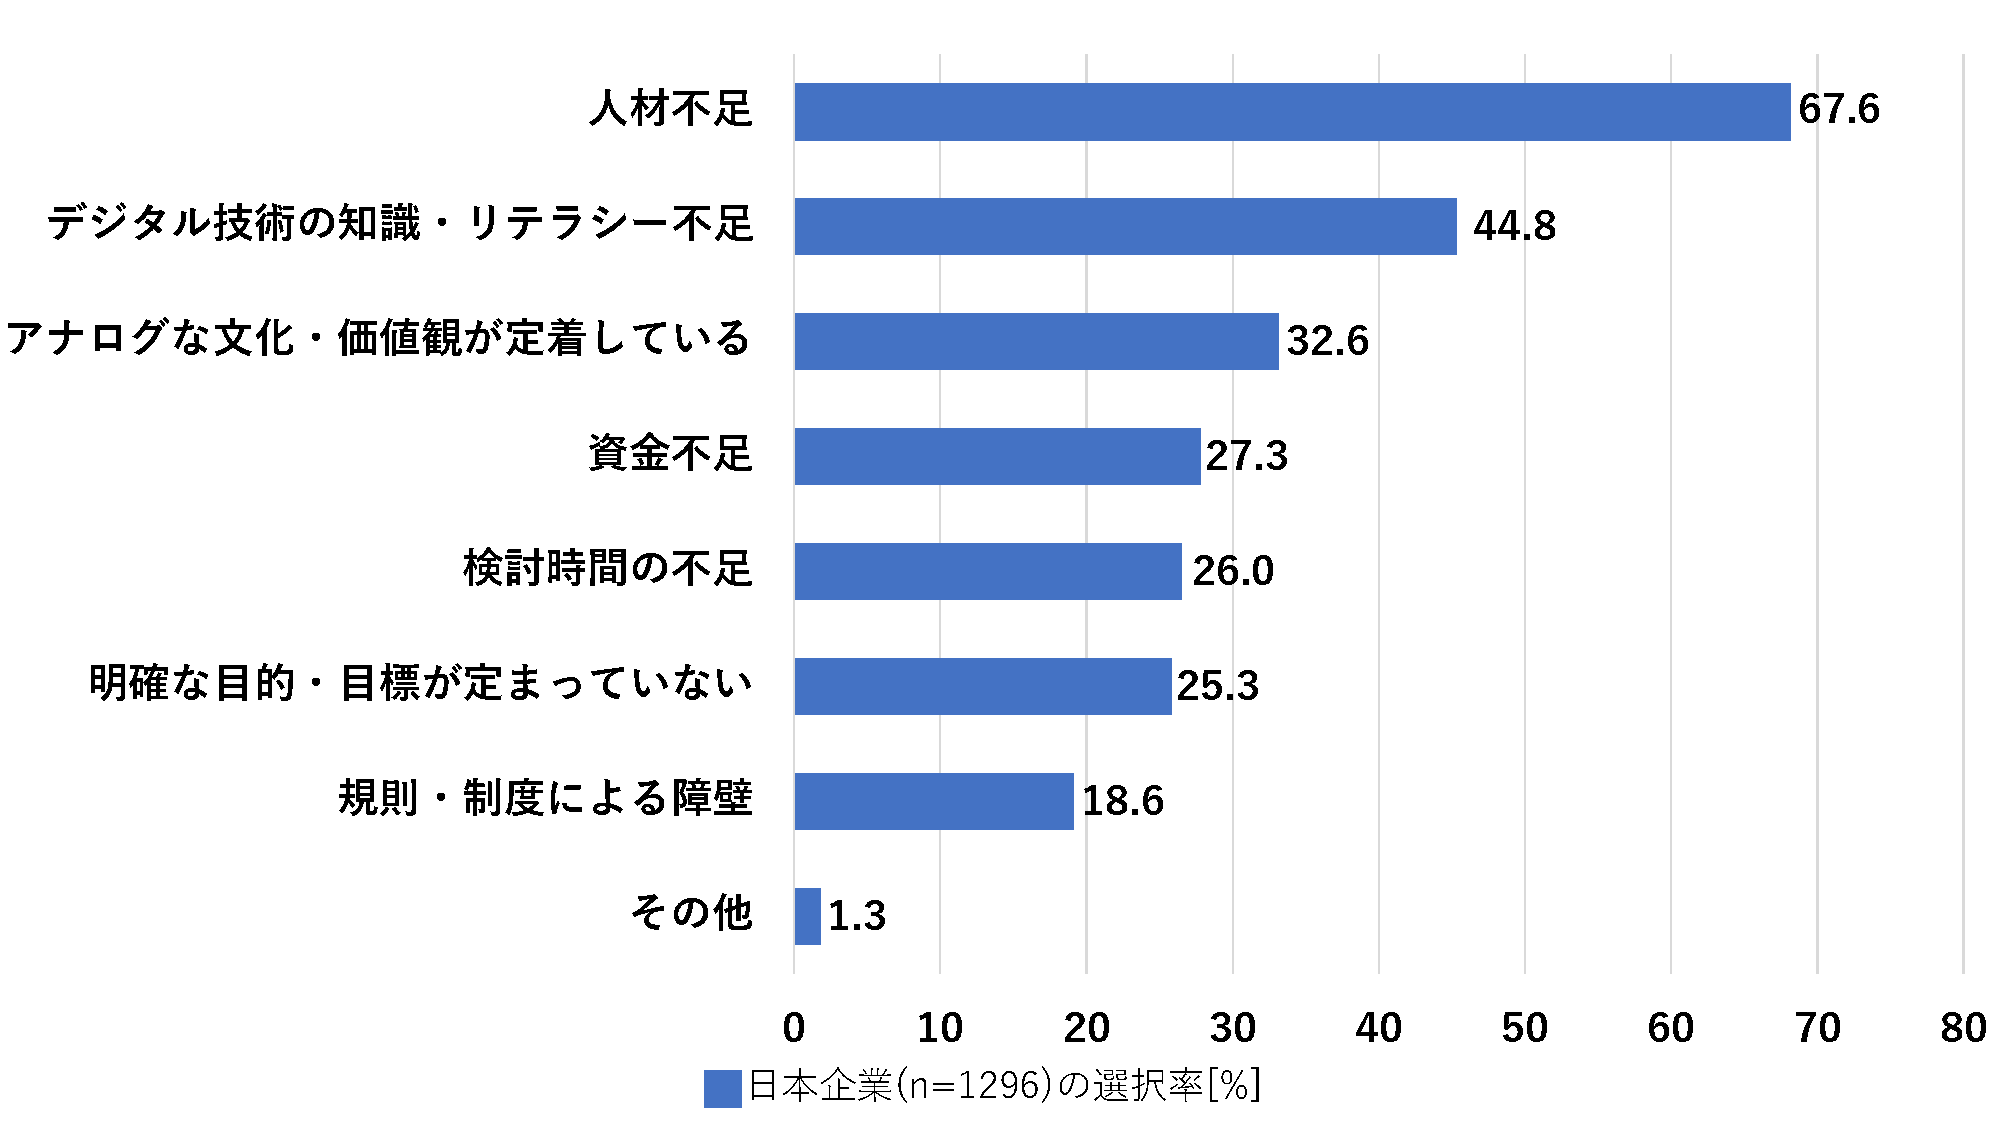
\includegraphics[clip,width=150mm]{figures/dx.pdf}
\caption[デジタル化を進める上での課題や障壁]{デジタル化を進める上での課題や障壁(複数選択)\linebreak}
\label{fig:dx}
\end{figure}

\clearpage

\section{情報教育について}%<3章>
本章では,現在の情報教育とネットワーク通信の学習について説明する.
\subsection{概要}
情報教育とは,子どもたちの情報活用能力の育成を図るものである.情報活用能力とは,「情報及び情報手段を主体的に選択し,活用していくための個人の基礎的な力」である.
情報教育の目標は以下の3つの観点に整理される\cite{kyoiku_gaiyou}.

\begin{enumerate}

\item[1] 情報活用の実践力\mbox{}\\
課題や目的に応じて情報手段を適切に活用すること\\
必要な情報を主体的に収集,判断,表現,処理,創造し,受け手の状況などを踏まえて発信,伝達できる能力

\item[2] 情報の科学的な理解\mbox{}\\
情報活用の基礎となる情報手段の特性の理解\\
情報を適切に扱うこと,自らの情報活用を評価,改善するための基礎的な理論や方法の理解

\item[3] 情報社会に参画する態度\mbox{}\\
社会生活の中で,情報や情報技術が果たしている役割や及ぼしている影響を理解し,情報モラルの必要性や情報に対する責任について考え,望ましい情報社会の創造に参画しようとする態度

\end{enumerate}
 上記の目標を達成するために,情報活⽤能⼒を⾔語能⼒と同様に学習の基盤となる資質・能⼒と位置付け,小学校,中学校,高等学校と段階的に学習していく.
 現在の情報教育の流れを図\ref{fig:kyouiku}に示す.
\\
\begin{figure}[h]
\centering
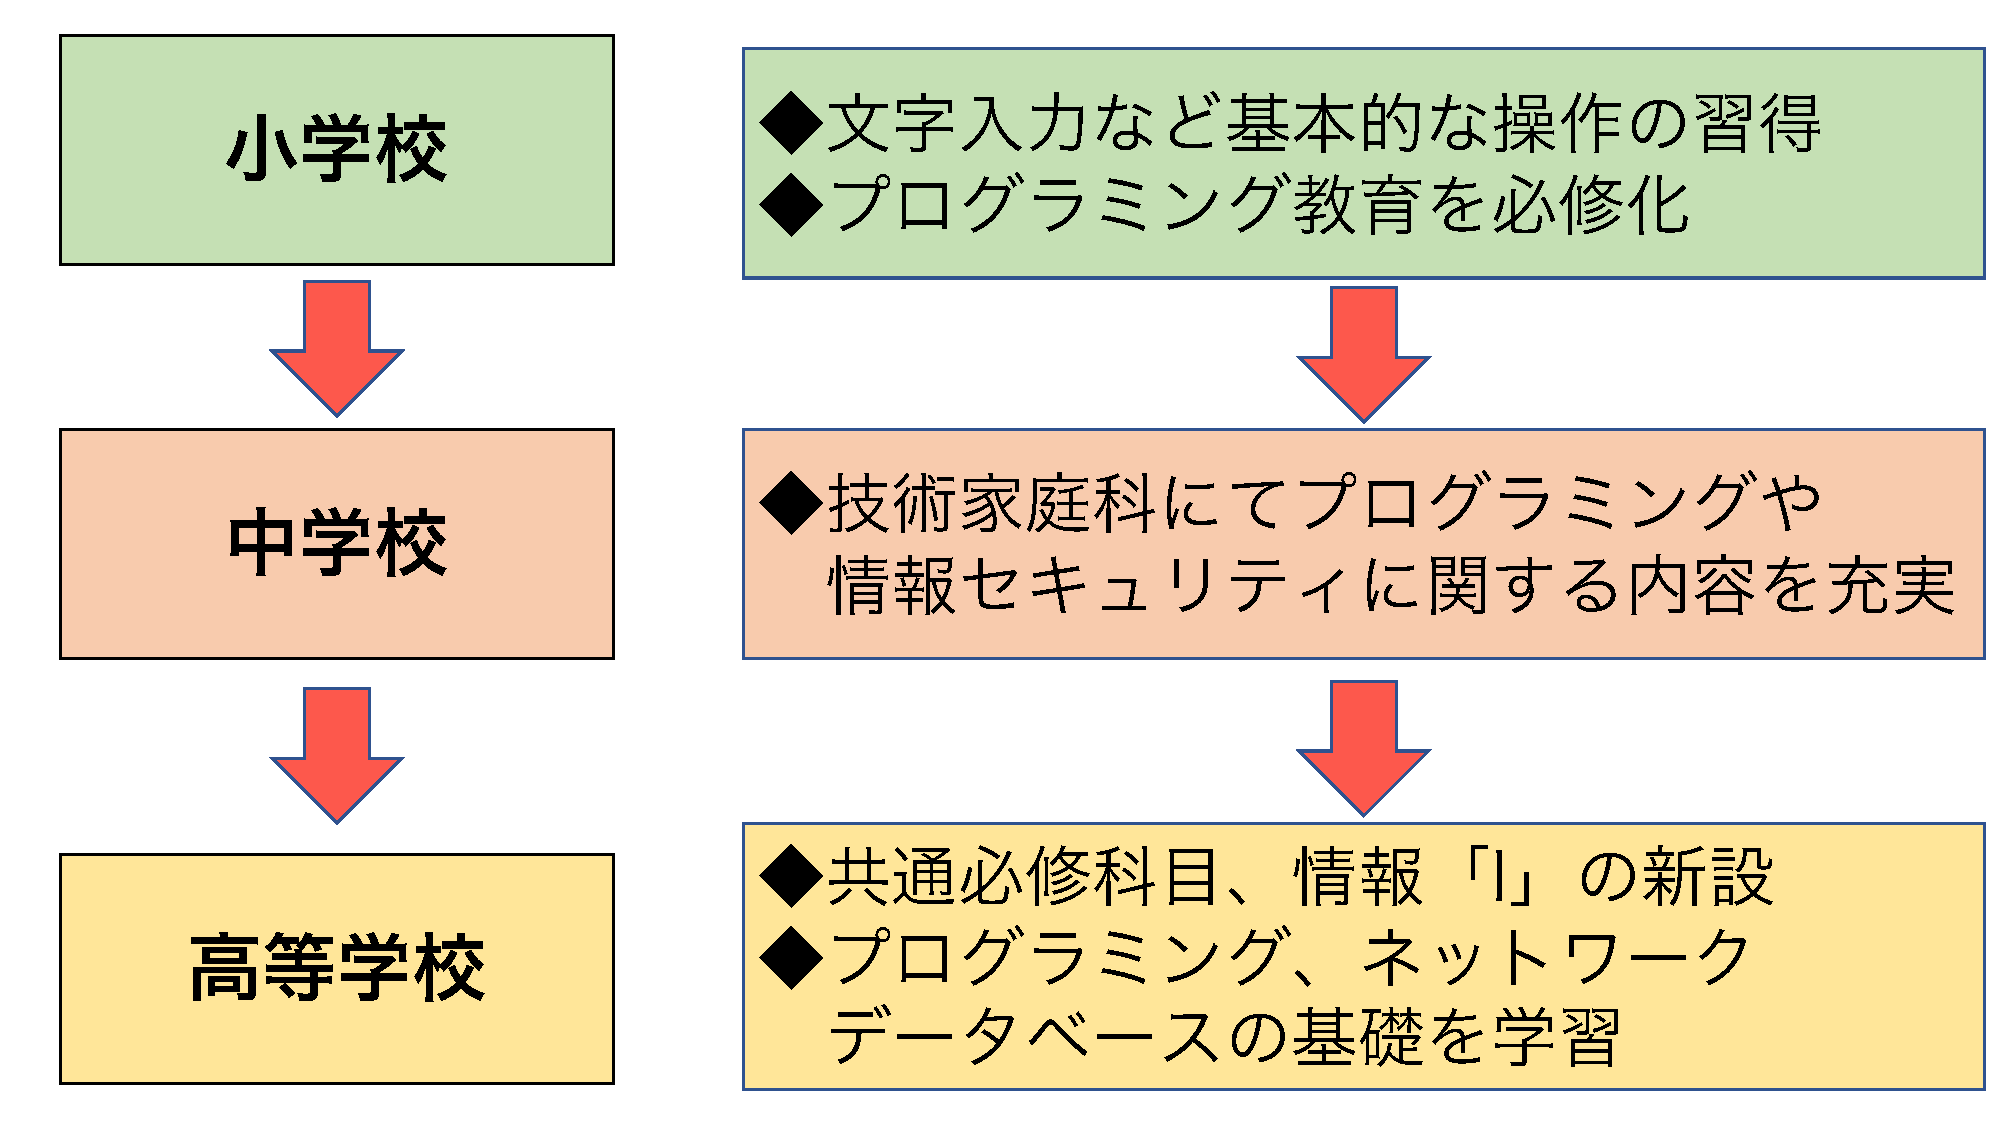
\includegraphics[clip,width=150mm]{figures/kyouiku.pdf}
\caption[現在の情報教育の流れ]{現在の情報教育の流れ\linebreak}
\label{fig:kyouiku}
\end{figure}

\clearpage

\subsection{小学校プログラミング教育}
\subsubsection{概要}
コンピュータ等を活用することが求められるこれからの社会では,コンピュータを理解し,活用していく力を身に付けることは,どのような職業に就くとしても極めて重要である.
そこで,導入されたのが小学校プログラミング教育である\cite{syogaku_pro}.

小学校プログラミング教育は,学習指導要領において「学習の基盤となる資質・能力」と位置付けられた「情報活用能力」の育成や情報手段(ICT)を「適切に活用した学習活動の充実」を進める中に,適切に位置付けられる必要がある.
よって,小学校プログラミング教育のねらいは情報教育の目標3つに対応した以下の3つに整理される.
\begin{enumerate}

\item[①] プログラミング的思考を育む\mbox{}\\
 プログラミング的思考とは,自分が意図する活動を実現するためにどのような動きの組み合わせが必要であり、一つ一つの動きの組合わせをどのように改善していくべきかなどを論理的に考えていく力のことである.

\item[➁] 身近な生活でコンピュータが活用されていること,問題解決に必要な手順があることに気づく\mbox{}\\
 コンピュータはプログラムで動いていることや,コンピュータに意図した処理を行わせるためには手順が必要なことなどの「気づき」が重要である.
そして,「気づき」をもとにコンピュータをより良い人生や社会を築くことといった,主体的に取り組む態度を涵養する.

\item[③] 各教科等の中で実施する場合については,「教科等での学びをより確実なものにする」こと\mbox{}\\
 小学校プログラミング教育は,新しい教科としてではなく既存の授業の中でプログラミングを学んでいく.
学習指導要領に例示されているものとして,小学校5年生の算数の多角形や,小学校6年生の理科の電流がつくる磁力などの単元でビジュアル言語を利用したプログラミングによって,法則や仕組みを体験的に学習することが出来る\cite{syogaku_jirei}.プログラムの例を図\ref{fig:syoupro}に示す.
\end{enumerate}

\clearpage

\begin{figure}[h]
\centering
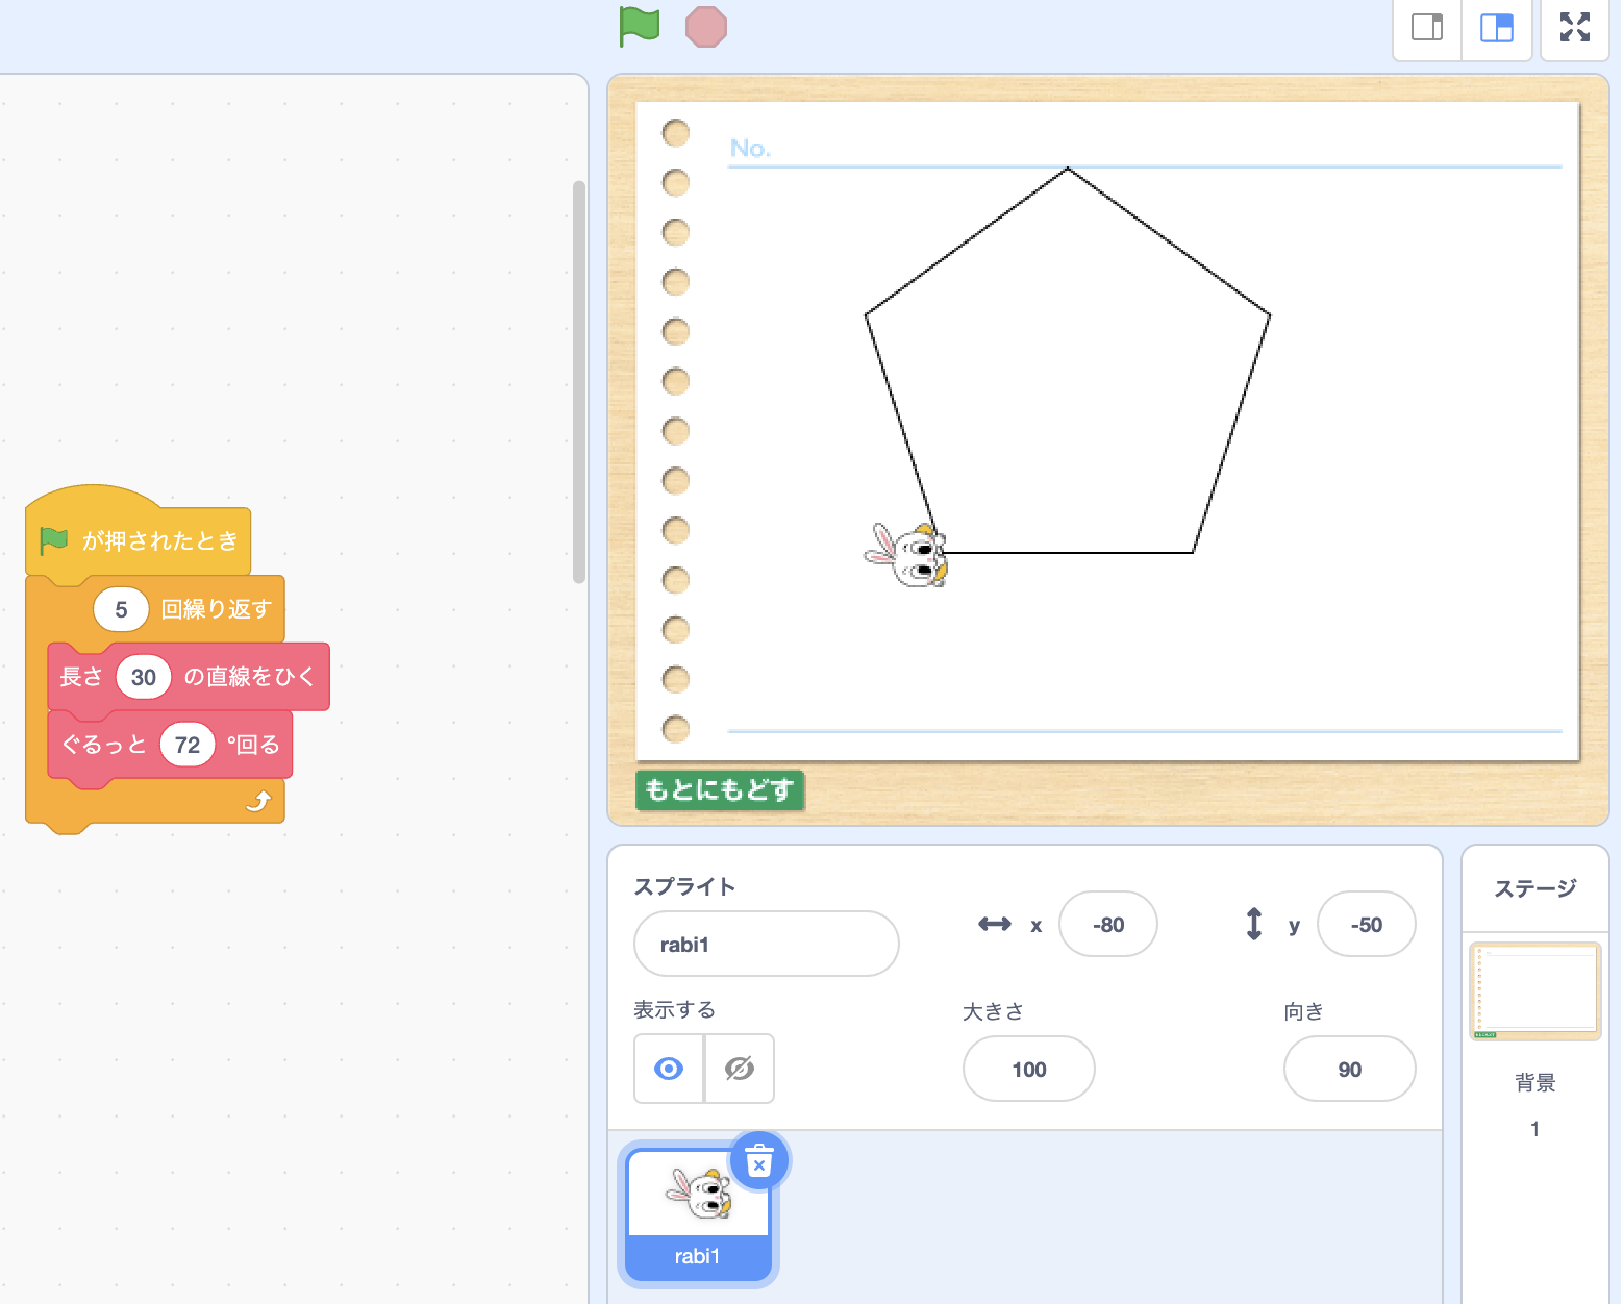
\includegraphics[clip,width=150mm]{figures/syoupro.pdf}
\caption[ビジュアル言語を利用したプログラミング例]{小学校プログラミング教育で行われるビジュアル言語を利用したプログラミング例\linebreak}
\label{fig:syoupro}
\end{figure}

 しかし,実際にどの授業にプログラミング教育を取り入れるか,使用するプログラミング言語や教材をどうするかは個々の小学校に委ねられている.
\subsubsection{小学校プログラミング教育におけるネットワーク通信の学習内容}
情報教育は,小学校,中学校,高等学校と段階的に行われる.一番最初である小学校プログラミング教育は,マウス操作やタイピング,ファイル操作のようなコンピュータに慣れ親しませるという段階から始まる.
また,小学校プログラミング教育はプログラミングから情報活用能力の育成を目指しているが,児童がプログラミング言語を覚えることやプログラミングの技能を習得すること自体はねらいとしていない.
したがって,情報技術に関する知識や技能に関する詳しい学習は中学校の段階から始まる.

\clearpage

\subsection{中学校技術・家庭科(技術分野)内容「D 情報の技術」}
\subsubsection{概要}
平成29年に告示された学習指導要領において,中学校では2021年度からプログラミング教育が必修化されることが公表され,
中学校技術・家庭科(技術分野)に元々存在していた「D 情報に関する技術」が「D 情報の技術」に変わり,指導内容が改められた\cite{tyugaku_29sidou}.
平成29年中学校学習指導要領の「D 情報の技術」の指導内容を以下に抜粋する.
\begin{enumerate}

\item[(1)] 生活や社会を支える情報の技術について調べる活動などを通して,次の事項を身に付けることができるよう指導する.
\begin{enumerate}
\item[(1)-ア] 情報の表現,記録,計算,通信の特性等の原理・法則と,情報のデジタル化や処理の自動化,システム化,情報セキュリティ等に関わる基礎的な技術の仕組み及び情報モラルの必要性について理解すること.

\item[(1)-イ] 技術に込められた問題解決の工夫について考えること.
\end{enumerate}

\item[(2)] 生活や社会における問題を,ネットワークを利用した双方向性のあるコンテンツのプログラミングによって解決する活動を通して,次の事項を身に付けることができるよう指導する.
\begin{enumerate}
\item[(2)-ア] 情報通信ネットワークの構成と,情報を利用するための基本的な仕組みを理解し,安全・適切なプログラムの制作,動作の確認及びデバッグ等ができること.

\item[(2)-イ] 問題を見いだして課題を設定し,使用するメディアを複合する方法とその効果的な利用方法等を構想して情報処理の手順を具体化するとともに,制作の過程や結果の評価,改善及び修正について考えること.
\end{enumerate}

\item[(3)] 生活や社会における問題を,計測・制御のプログラミングによって解決する活動を通して,次の事項を身に付けることができるよう指導する.
\begin{enumerate}
\item[(3)-ア] 計測・制御システムの仕組みを理解し,安全・適切なプログラムの制作,動作の確認及びデバッグ等ができること.

\item[(3)-イ] 問題を見いだして課題を設定し,入出力されるデータの流れを元に計測・制御システムを構想して情報処理の手順を具体化するとともに,制作の過程や結果の評価,改善及び修正について考えること.
\end{enumerate}

\item[(4)] これからの社会の発展と情報の技術の在り方を考える活動などを通して,次の事項を身に付けることができるよう指導する.
\begin{enumerate}
\item[(4)-ア] 生活や社会,環境との関わりを踏まえて,技術の概念を理解すること.

\item[(4)-イ] 技術を評価し,適切な選択と管理・運用の在り方や,新たな発想に基づく改良と応用について考えること.
\end{enumerate}
\end{enumerate}

学習指導要領の改訂によって,小学校プログラミング教育の成果を生かし発展させ,高等学校「情報Ⅰ」への接続を意識する方針となっている.
具体的には,従前からの計測・制御に加えて,ネットワークを利用した双方向性のあるコンテンツのプログラミングについても取り上げられる.
また,情報通信ネットワークやセキュリティ、情報モラルについても充実する.

中学校では教科として情報教育が行われるようになったが,授業で使用するプログラミング言語や教材は個々の中学校に委ねられている.
教科書によって利用される言語は異なり,ビジュアル型言語である「Scratch」のみを使用するもの\cite{tyugaku_kyo1},「Scratch」と日本語入力型テキスト言語の「なでしこ」を併用するもの\cite{tyugaku_kyo2},ビジュアル型とテキスト型を切り替えられるものなどがある\cite{tyugaku_kyo3}.
\subsubsection{中学校技術・家庭科におけるネットワーク通信の学習内容}
中学校技術・家庭科におけるネットワーク通信の学習は,「D 情報の技術」の(1) 生活や社会を支える技術の授業で行われる.
情報通信ネットワークの仕組みや特徴と関連付けて,情報セキュリティや情報モラルの必要性を学習するという流れである.
「D 情報の技術」の教員研修用教材をもとに,中学校におけるネットワーク通信に関する学習の内容を以下に示す\cite{tyugaku_kensyu}.
\begin{enumerate}

\item[A] インターネットとは\mbox{}\\
 ネットワークの意味や,LAN(Local Area Network)とWAN(Wide Area Network)について,TCP/IPというプロトコルがあること,インターネットが分散型ネットワークであることを学習する.

\item[B] パケット通信\mbox{}\\
 データを分割して送信し受信側で元のデータに組み立て直すこと,分割したデータをラベル付けして宛先を認識すること,適切な経路を認識し渋滞を避けることなどを学習する.

\item[C] IP アドレス,MAC アドレス,DHCP サーバ\mbox{}\\
 インターネット上の端末には住所としてIPアドレスが割り振られていること,IPアドレスにはプライベートアドレスとグローバルアドレスとがあることを学習する.
 また,端末の個体を識別する番号をMACアドレスと呼び,MACアドレスを利用してDHCPサーバというものがIPアドレスを割り振っていることを学習する.
\item[D] DNS サーバ\mbox{}\\
 電子メールやWebサイトなどの人間にも分かりやすいアドレス表記のことをFQDNと呼ぶこと,FQDNからIPアドレスを調べるものがDNSサーバであることFQDNの名前からIPアドレスを特定していく仕組みを名前解決と呼ぶことなどを学習する.
\end{enumerate}

教員研修として行われた事例で\cite{tyugaku_kensyu2},ネットワーク通信の学習は,「ネットワークを利用した双方向性のあるコンテンツのプログラミングによる問題の解決」のテーマで演習を行う前の講義形式の授業で行われている.
講義を行った後に,ビジュアル言語を利用した擬似的な通信アプリケーションやWebページを作る演習が行われる.
実際に中学校で行われた授業事例では,ネットワーク通信の大まかな仕組みを学習後,メインの演習としてネットワークを活用したシステムやコンテンツをプログラミングによって作成し改善・修正案を話し合うという授業が多い\cite{tyugaku_jirei}.

\clearpage

\subsection{高校「情報Ⅰ」}
\subsubsection{概要}
高等学校については,平成30年に新しい学習指導要領が公示された.
共通教科情報科が改訂されたことにより\cite{koukou_sidou},共通必履修科目として「情報Ⅰ」が設けられ,発展的な選択科目として「情報Ⅱ」が設けられた.

以下に「情報Ⅰ」の学習目標を示す.
\begin{enumerate}

\item[a] 効果的なコミュニケーションの実現,コンピュータやデータの活用について理解を深め技能を習得するとともに,情報社会と人との関わりについて理解を深めるようにする\mbox{}\\
 効果的なコミュニケーションを実現するために必要な情報デザイン,情報が処理される仕組みを理解する.
また,データを活用するためにモデル化とシミュレーション,ネットワーク,データベースなどについて理解し,技能を身に付ける.
情報社会と人との関わりについては,情報に関する法規や制度及びマナーなどについて,情報技術の理解と併せて身に付けるようにする.
\\
\item[b] 様々な事象を情報とその結び付きとして捉え,問題の発見・解決に向けて情報と情報技術を適切かつ効果的に活用する力を養う\mbox{}\\
 情報に関する科学的な見方・考え方を働かせ,様々な事象を情報とその結び付きとして捉える.
また,コンピュータ,ネットワーク,データベースなどの活用を通して,情報社会などの問題の発見・解決に向けて試行錯誤を行い,情報技術を適切かつ効果的に活用する力を養うことようにする.
\\
\item[c] 情報と情報技術を適切に活用するとともに,情報社会に主体的に参画する態度を養う\mbox{}\\
 情報モラルを養い,情報と情報技術を活用することで情報社会に主体的に参画する態度を養うようにする.
 
\end{enumerate}

「情報Ⅰ」の内容を以下に示す.
\begin{enumerate}

\item[(A)] 情報社会の問題解決\mbox{}

\item[(B)] コミュニケーションと情報デザイン\mbox{}

\item[(C)] コンピュータとプログラミング\mbox{}

\item[(D)] 情報通信ネットワークとデータの活用\mbox{}
\end{enumerate}

共通教科情報科は,小・中・高等学校の各教科等の指導を通じて行われる情報教育の中核である.
よって,中学校の関連する教科等との縦の連携,高等学校の他教科等との横の連携も極めて重要であるとされている.
\clearpage
\subsubsection{高校「情報Ⅰ」におけるネットワーク通信の学習内容}
高校「情報Ⅰ」におけるネットワーク通信の学習は,(D)情報通信ネットワークとデータの活用で行われる.
(D)情報通信ネットワークとデータの活用のネットワーク通信に関わる学習内容を以下に示す.
\begin{enumerate}

\item[(D)-1] 情報通信ネットワークの仕組みや構成要素,プロトコルの役割及び情報セキュリティを確保するための方法や技術について理解すること.
\mbox{}\\
(D)-1では,コンピュータ同士を接続する仕組みや情報通信ネットワークを構成するクライアントやサーバ,ハブ,ルータなどの構成要素の役割について理解するようにする.
また,パケット通信やプロトコル,通信の階層構造,暗号化などについて理解するようにする.\\
 
\item[(D)-2] 目的や状況に応じて,情報通信ネットワークにおける必要な構成要素を選択するとともに,情報セキュリティを確保する方法について考えること.
\mbox{}\\
(D)-2では,家庭内LAN(Local Area Network)等の小規模な情報通信ネットワークの仕組みを取り上げ,情報通信ネットワークを構築するために必要な構成要素やプロトコル,ネットワークの設計について適切に選択する力を養うようにする.
\end{enumerate}
 高等学校においても,ネットワーク通信の仕組みについての学習は講義形式の授業が多いと考えられる.
教員向け研修用教材にある演習は\cite{koukou_kensyu},家や店舗など小規模のLANの構成を手描きや作図ソフトで描くことや,無線LANと有線LANのメリットやデメリットを話し合うなどである.
実践事例では\cite{koukou_jirei},無線LAN ルータ,スマートフォン,タブレットPCなどを用いて,簡単な無線LANの構築の実習を行いDHCPやIP アドレス,SSID(Service Set Identifier),暗号化キー(Wi-Fi パスワード)について学習している.
授業用コンテンツでは\cite{koukou_kon},動画,スライド,ワークシートを組み合わせてLANの構築や機器を学習する演習が公開されている.
研修用教材,実践事例,授業用コンテンツ全ての演習,実習がネットワークの構築についての学習である.したがって,パケット通信やプロトコル,通信の階層構造などの学習は講義形式で行われていると考えられる.
\clearpage
\subsection{ネットワーク通信の学習教材について}
\subsubsection{「情報Ⅰ」教科書付属の教材}
「情報Ⅰ」教科書付属の教材として,紙の教科書にあるQRコードを読み取るか,電子版の教科書であるデジタル教科書から利用できるアニメーション教材の例を図\ref{fig:kou_anime}に示す\cite{koukou_anime}.
\begin{figure}[h]
\centering
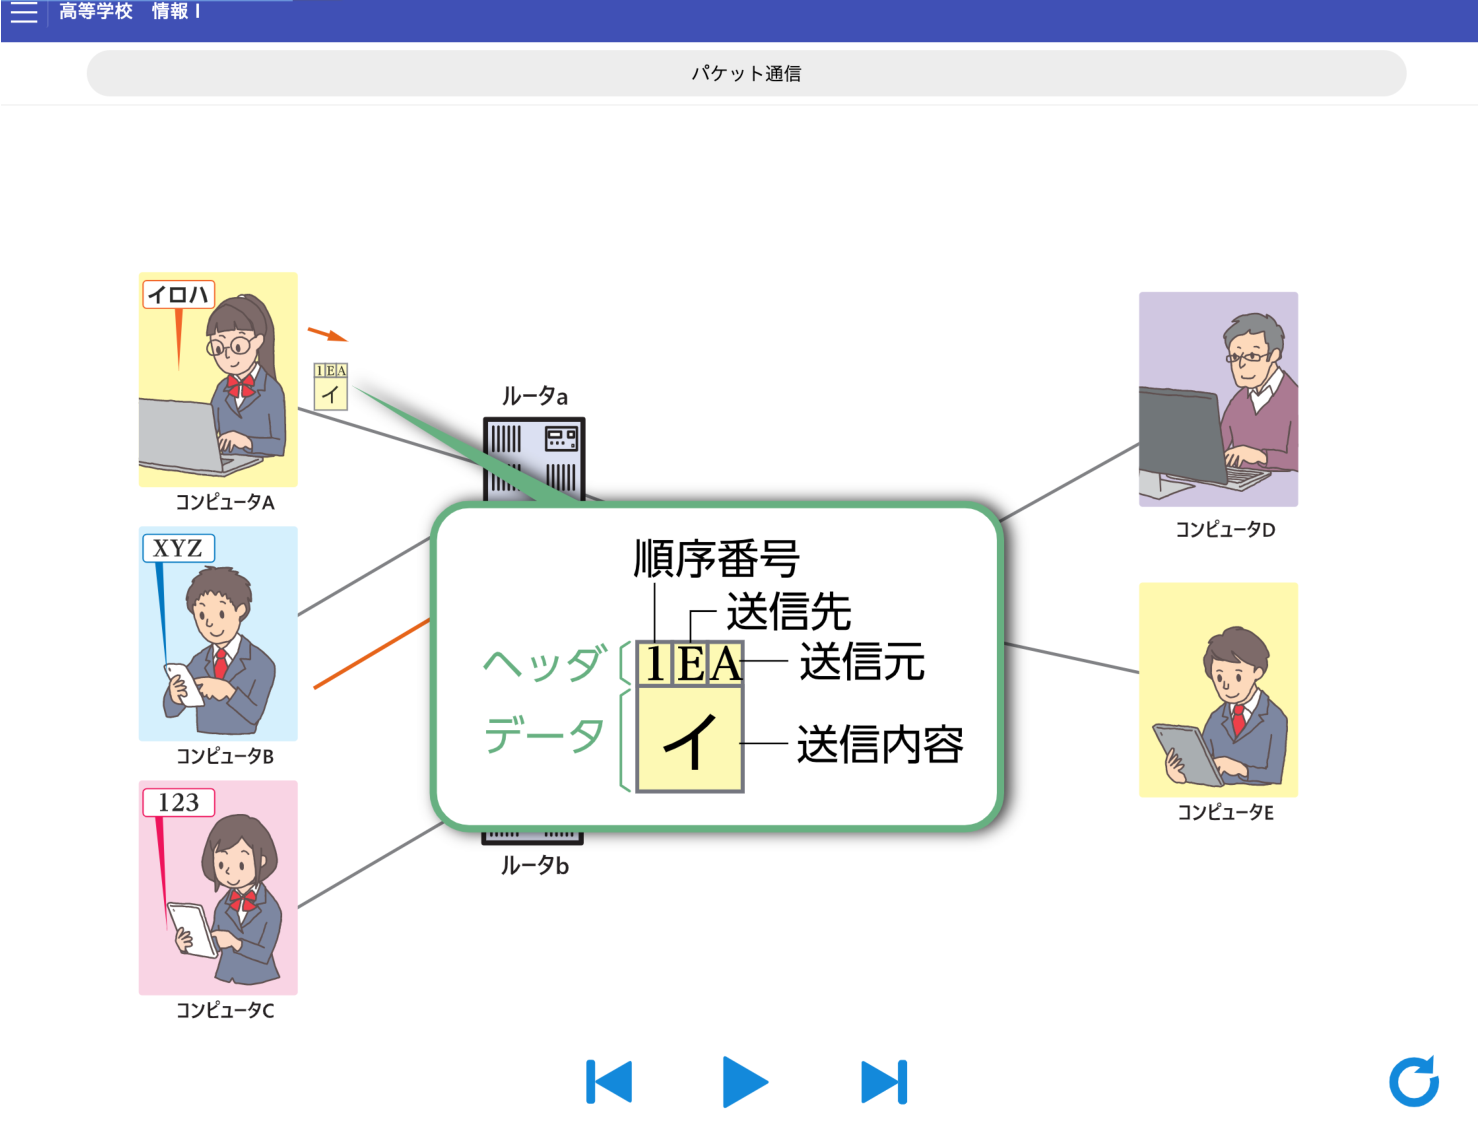
\includegraphics[clip,width=150mm]{figures/koukou_anime.pdf}
\caption[数研出版|高等学校 情報Ⅰ|パケット通信のコンテンツの画面]{数研出版|高等学校 情報Ⅰ|パケット通信のコンテンツの画面\linebreak}
\label{fig:kou_anime}
\end{figure}

このアニメーション教材はパケット通信を大まかに説明している.一連のアニメーションに,パケットの構造と分割やルータの機能,経路制御表の仕組みなどを詰め込んでいるため,細かな解説が難しくなったと考えられる.
このようなQRコードからアクセスできるコンテンツは,つまずきやすい学習内容の補助や自宅学習を助ける資料として作られている\cite{koukou_qr}.
しかし,多くの教科書にネットワーク通信の階層構造を学習するコンテンツが存在していない.
また,教科書によってはパケット通信を解説するコンテンツすら無い場合がある\cite{koukou_kyokasyo}.
共通鍵暗号方式やパリティチェックなどの暗号化の学習が優先されているが,学習指導要領にはネットワーク通信の階層構造の理解も含まれており,教科書の文字や図だけで階層ごとの機能や違いを理解することは難しいと考えられる.

\clearpage

\subsubsection{「情報Ⅰ」動画教材}
「情報Ⅰ」の学習教材として,一般社団法人である情報処理学会が設置している動画教材「IPSJ MOOC」がある\cite{koukou_douga1}.
この動画教材は,教員研修や児童・生徒・学生による自己学習,授業などでの利用を目的として作成された.
「情報Ⅰ」の学習内容を全体的に解説する動画で,学習内容ごとに細かく分割されている.
情報通信ネットワークの仕組みと役割のテーマが存在し,LAN,通信プロトコル,暗号化の順に学習していく.
通信プロトコルを学習する動画内の,ネットワーク通信の階層構造を解説している場面を図\ref{fig:kou_douga}に示す\cite{koukou_douga2}.

\begin{figure}[h]
\centering
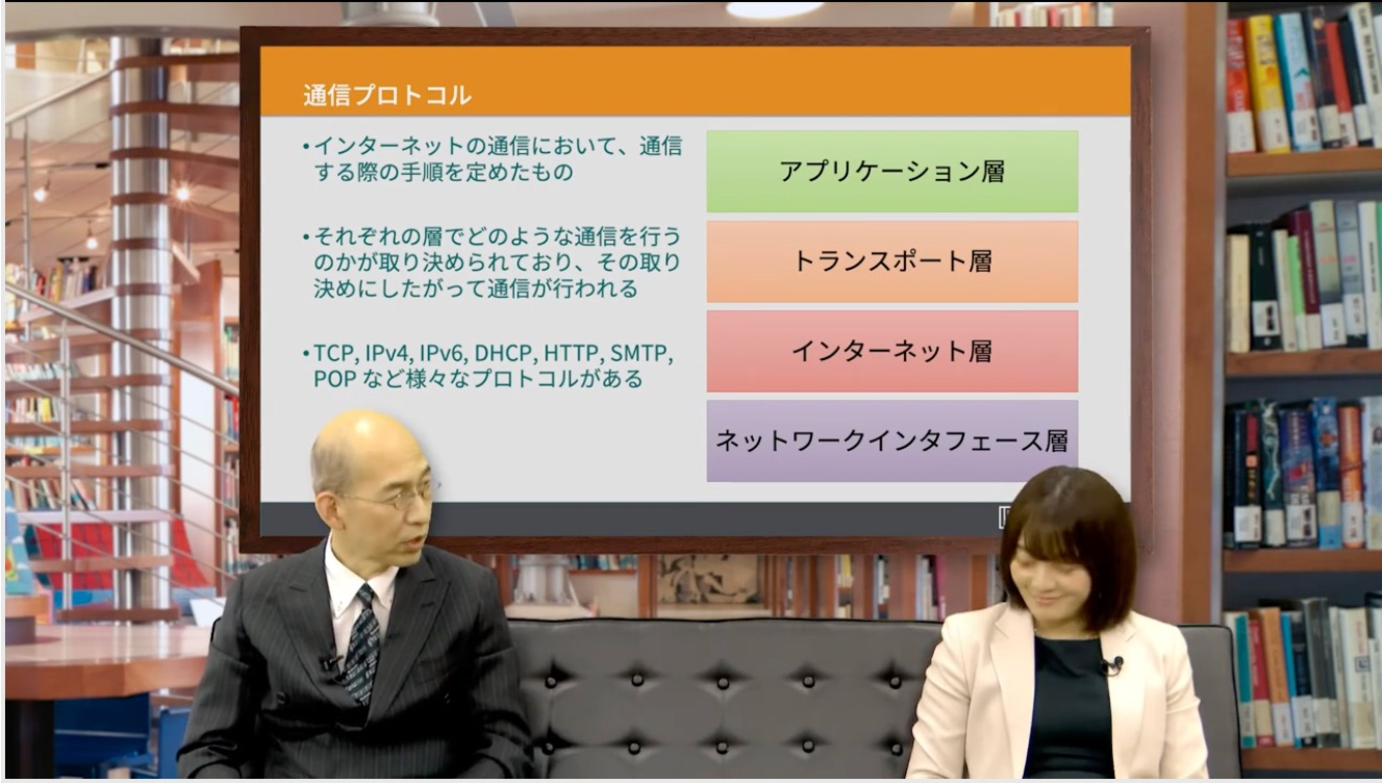
\includegraphics[clip,width=150mm]{figures/koudouga.pdf}
\caption[IPSJ MOOC2. 情報通信ネットワークの仕組み②通信プロトコルの動画教材]{IPSJ MOOC 2. 情報通信ネットワークの仕組み②通信プロトコルの動画教材の一部\linebreak}
\label{fig:kou_douga}
\end{figure}

全ての動画の形式として,高校や大学の教員,教授が対話しながら進行する教育番組のようなストーリー形式である.
「情報Ⅰ」の学習内容ではあるが,小学生や中学生の利用も配慮されているためこのような形式になったと考えられる.
ネットワーク通信の階層構造を解説する場面では,全体の階層構造は紹介されるものの,階層ごとの説明は図やアニメーションで示されず口頭のみでの解説である.
したがって,この教材で階層ごとの機能や違いを理解することは難しいと考えられる.
\clearpage

\section{ネットワークの基礎知識}%<4章>
本章では,作成したWeb教材で学習する基礎知識について説明する.
\subsection{OSI}
\subsubsection{概要}
OSI(Open Systems Interconnection)とは,国際標準化機構ISO( International Organization for Standardization)と国連機関ITU-T(International Telecommunication Union Telecommunication Standardization Sector)により1982年に国際標準として策定が開始された通信体系である.
OSIの策定が進められる中で,TCP/IPやイーサネットに準拠した製品が普及し始めており,OSIによって定められたOSIプロトコルは複雑で実装が困難であったため,普及しなかった.
\subsubsection{OSI参照モデル}
OSI参照モデルとは,ネットワーク通信で利用されるプロトコルをを7つの階層に分類したモデルである.
図\ref{fig:osi}に構造を示す.

\begin{figure}[h]
\centering
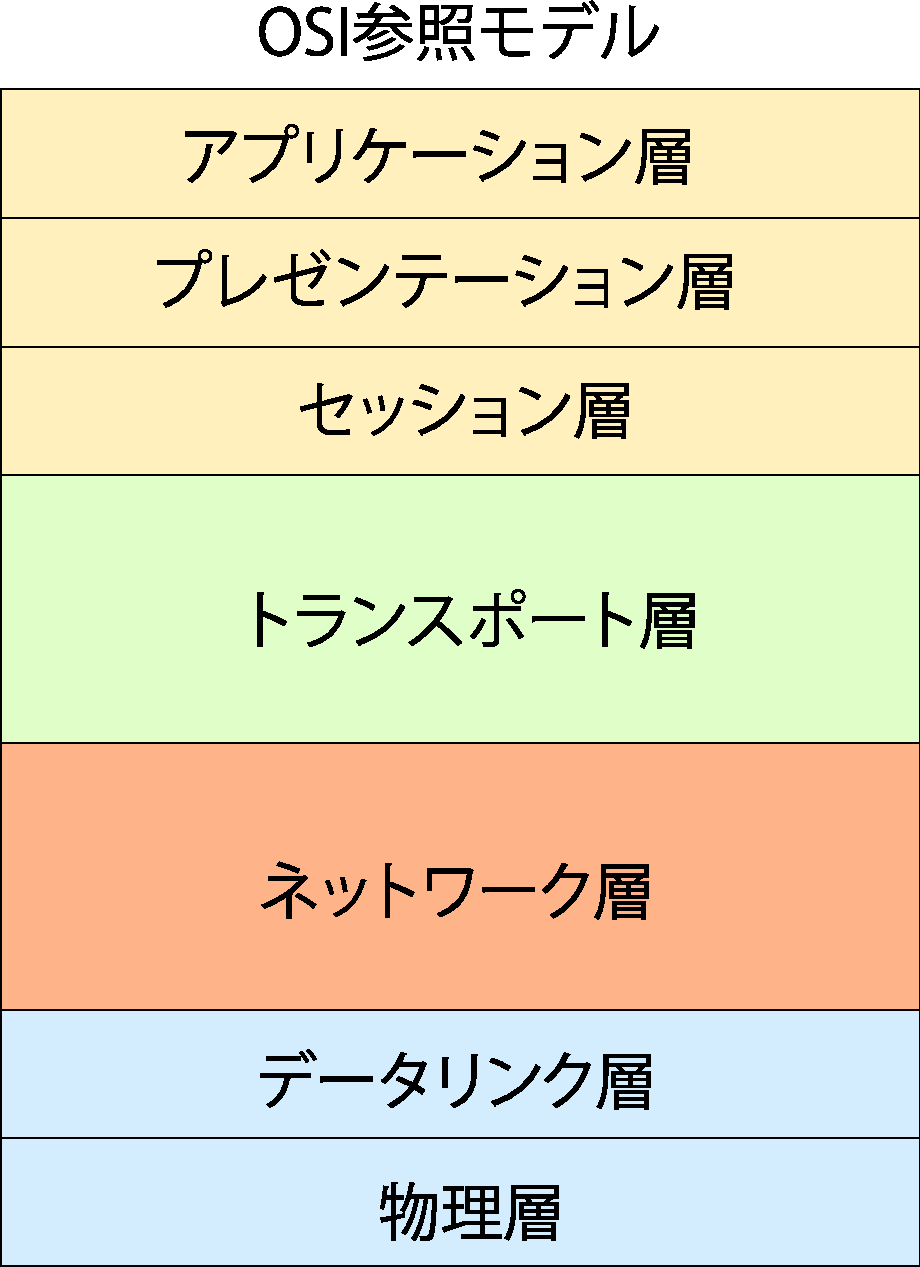
\includegraphics[clip,width=70mm]{figures/osi.pdf}
\caption[OSI参照モデル]{OSI参照モデル\linebreak}
\label{fig:osi}
\end{figure}

OSI参照モデルとTCP/IPの階層モデルは対応しているわけではないが,対応づけすることで理解を助けるとして教科書や参考書で利用されている.
本研究で作成したWeb教材も同様に,OSI参照モデルをTCP/IPの構造に当てはめることでTCP/IPの仕組みが分かりやすくなることを想定して作成している.
\subsection{TCP/IP}
\subsubsection{概要}
TCP/IP(Transmission Control Protocol / Internet Protocol)とは,現在のインターネットを含む多くのコンピュータで構成されるネットワークにおいて,世界標準的に利用されている通信プロトコルのセットである.
インターネットプロトコルスイート(Internet protocol suite)とも呼ばれている.
TCP/IPは,1970年代初期にアメリカの軍用ネットワーク用の次世代プロトコルの研究から開発され,最初の仕様は1974年に公開された.
1980年代前半に,TCP/IPを標準サポートしたUnix系のOSが公開され教育・研究機関によりTCP/IPによるネットワークの構築が進み,TCP/IPによる世界的なネットワークをインターネットと呼ぶようになった.
1991年にWWW(World Wide Web)というインターネット上のコンテンツ同士を結びつけるシステムが公開されwebが普及し始めた.
webの利用にはTCP/IPを標準サポートしたOSが必要であり,1994年以降にTCP/IPを標準サポートした一般企業・ユーザ向けOSが登場したためTCP/IPが世界的に一気に普及することになった.
\subsubsection{TCP/IPの階層}
TCP/IPの階層モデルを図\ref{fig:tcpip_sou}に示す.

\begin{figure}[h]
\centering
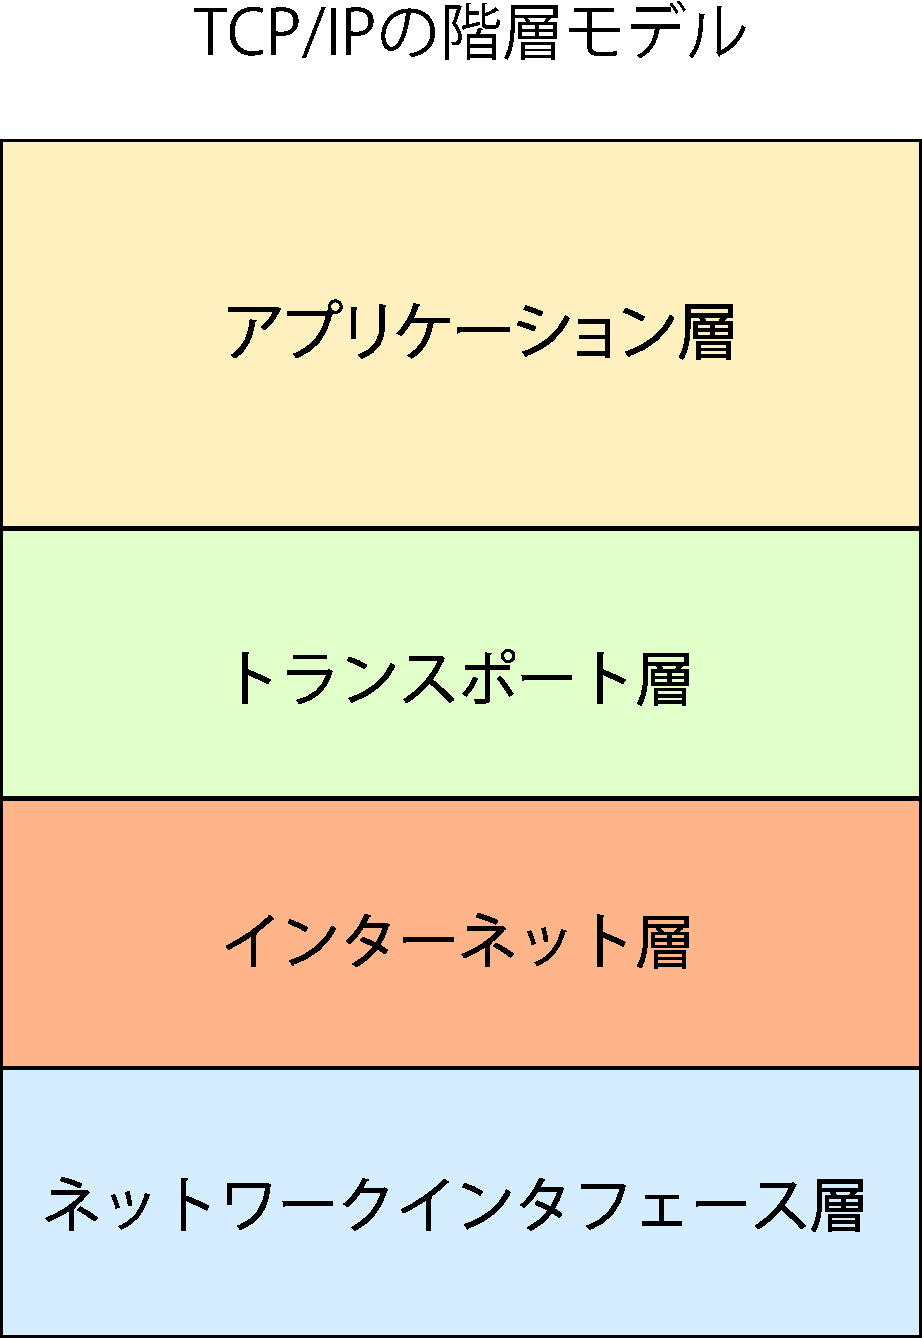
\includegraphics[clip,width=70mm]{figures/TCPIPmodel.pdf}
\caption[TCP/IPの階層モデル]{TCP/IPの階層モデル\linebreak}
\label{fig:tcpip_sou}
\end{figure}

TCP/IPはOSI参照モデルと同じように、役割を階層に分けている.
同じ名前の階層もあるが,TCP/IPの階層モデルとOSI参照モデルが完全に対応しているわけでは無い.
データを送信する際は、上位層から下位層へデータを渡しヘッダを付与していく.
この仕組みををカプセル化と呼ぶ.
また,データとヘッダのまとまりをパケットと呼ぶ.
アプリケーションが通信を行う際は,データを分割しパケットとしてそれぞれカプセル化して送信する.
パケット送信時のカプセル化の例を図\ref{fig:capu}に示す.
\clearpage
\begin{figure}[h]
\centering
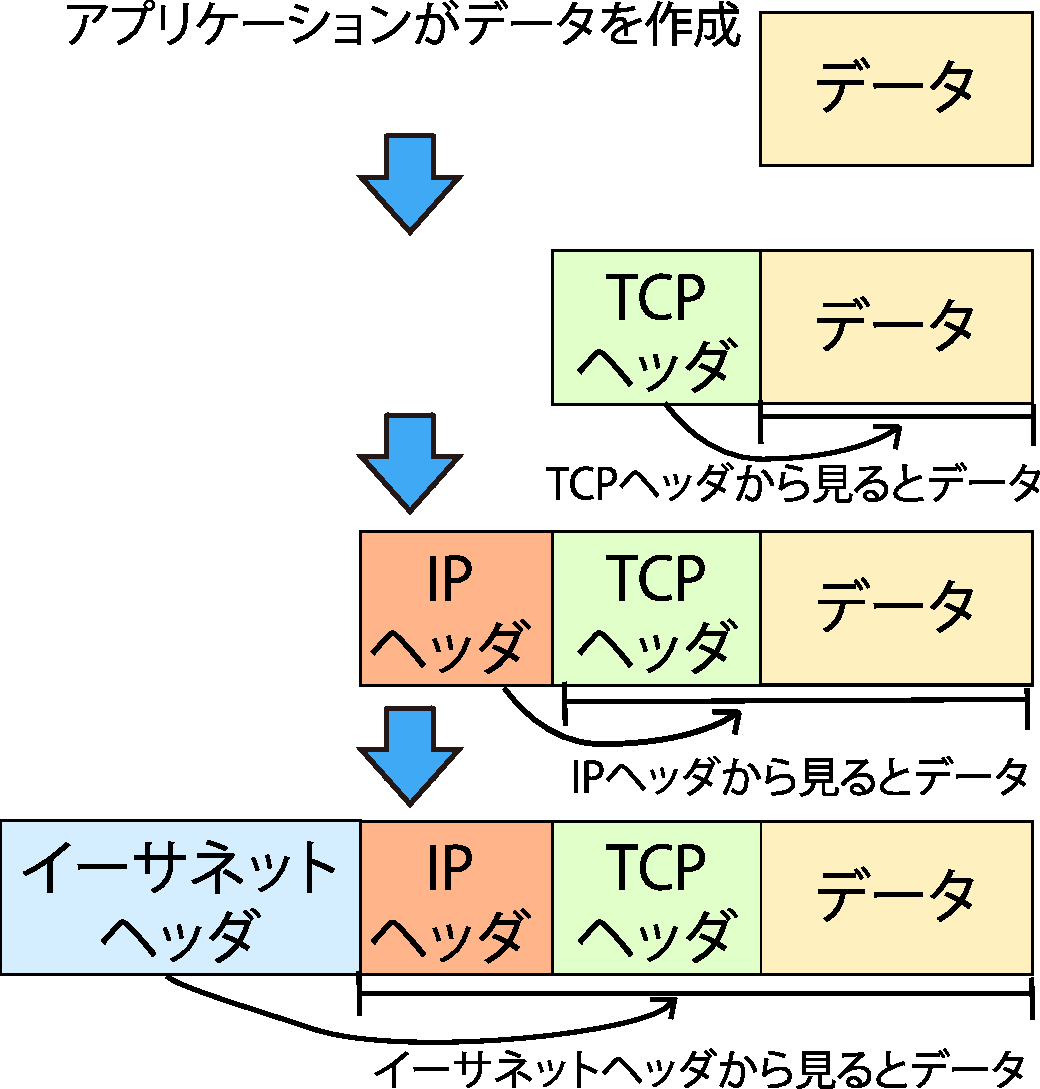
\includegraphics[clip,width=95mm]{figures/capu.pdf}
\caption[パケット送信時のカプセル化の概略図]{パケット送信時のカプセル化の概略図\linebreak}
\label{fig:capu}
\end{figure}

受信時は送信時とは逆に,図\ref{fig:capu2}に示すように下位層から上位層にヘッダを除去しながらデータを渡していく.

\begin{figure}[h]
\centering
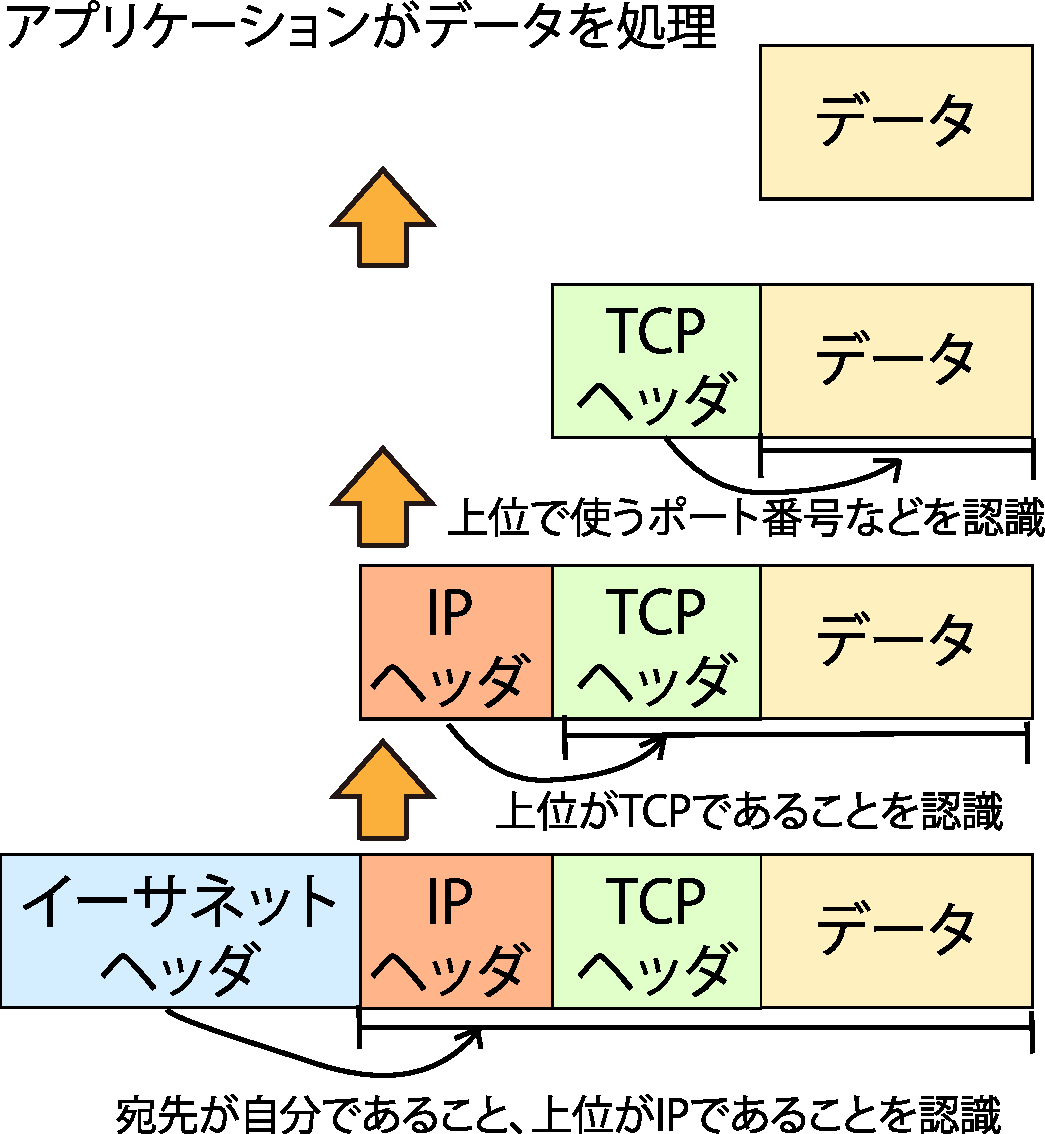
\includegraphics[clip,width=95mm]{figures/capu2.pdf}
\caption[パケット受信時のヘッダ除去の概略図]{パケット受信時のヘッダ除去の概略図\linebreak}
\label{fig:capu2}
\end{figure}

\subsection{データリンク層とネットワーク層}
データリンク層とネットワーク層とは,OSI参照モデルの層である.
図\ref{fig:kaisou}に示すように,TCP/IPの階層ではインターネット層とネットワークインタフェース層にあたる.
\\
\begin{figure}[h]
\centering
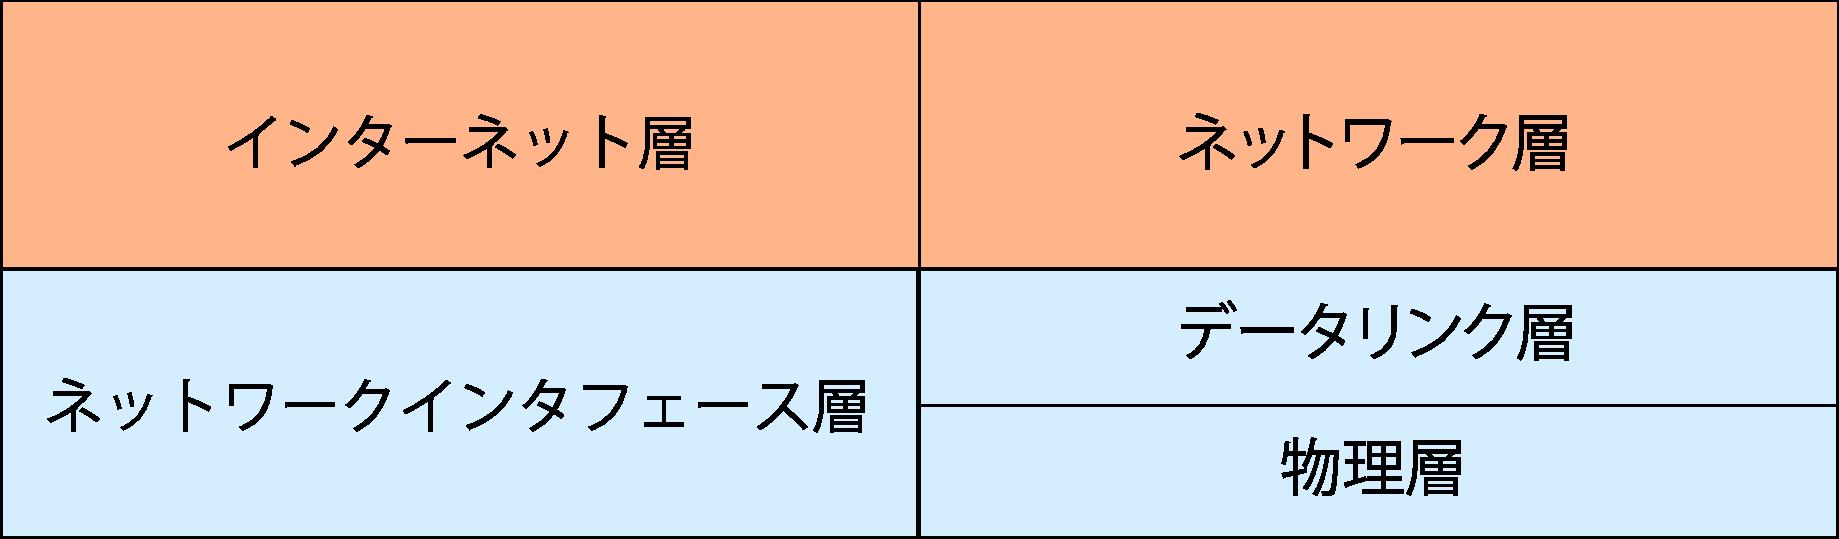
\includegraphics[clip,width=95mm]{figures/kaisou.pdf}
\caption[下位層におけるOSI参照モデルとTCP/IPの対応]{下位層におけるOSI参照モデルとTCP/IPの対応\linebreak}
\label{fig:kaisou}
\end{figure}

これらの層は,コンピュータ同士のデータ伝送を実現している.
しかし,ネットワーク層はエンドツーエンド(end-to-end)と呼ばれる終点ノード間の通信を実現し,データリンク層は同じ種類の通信手段で接続されているノード間の通信を実現する.
つまり,ネットワーク層は始点と終点の通信を,データリンク層は始点と終点の間の1区間ごとの通信を提供する.
違いを単純化したようすを図に示す.

\begin{figure}[h]
\centering
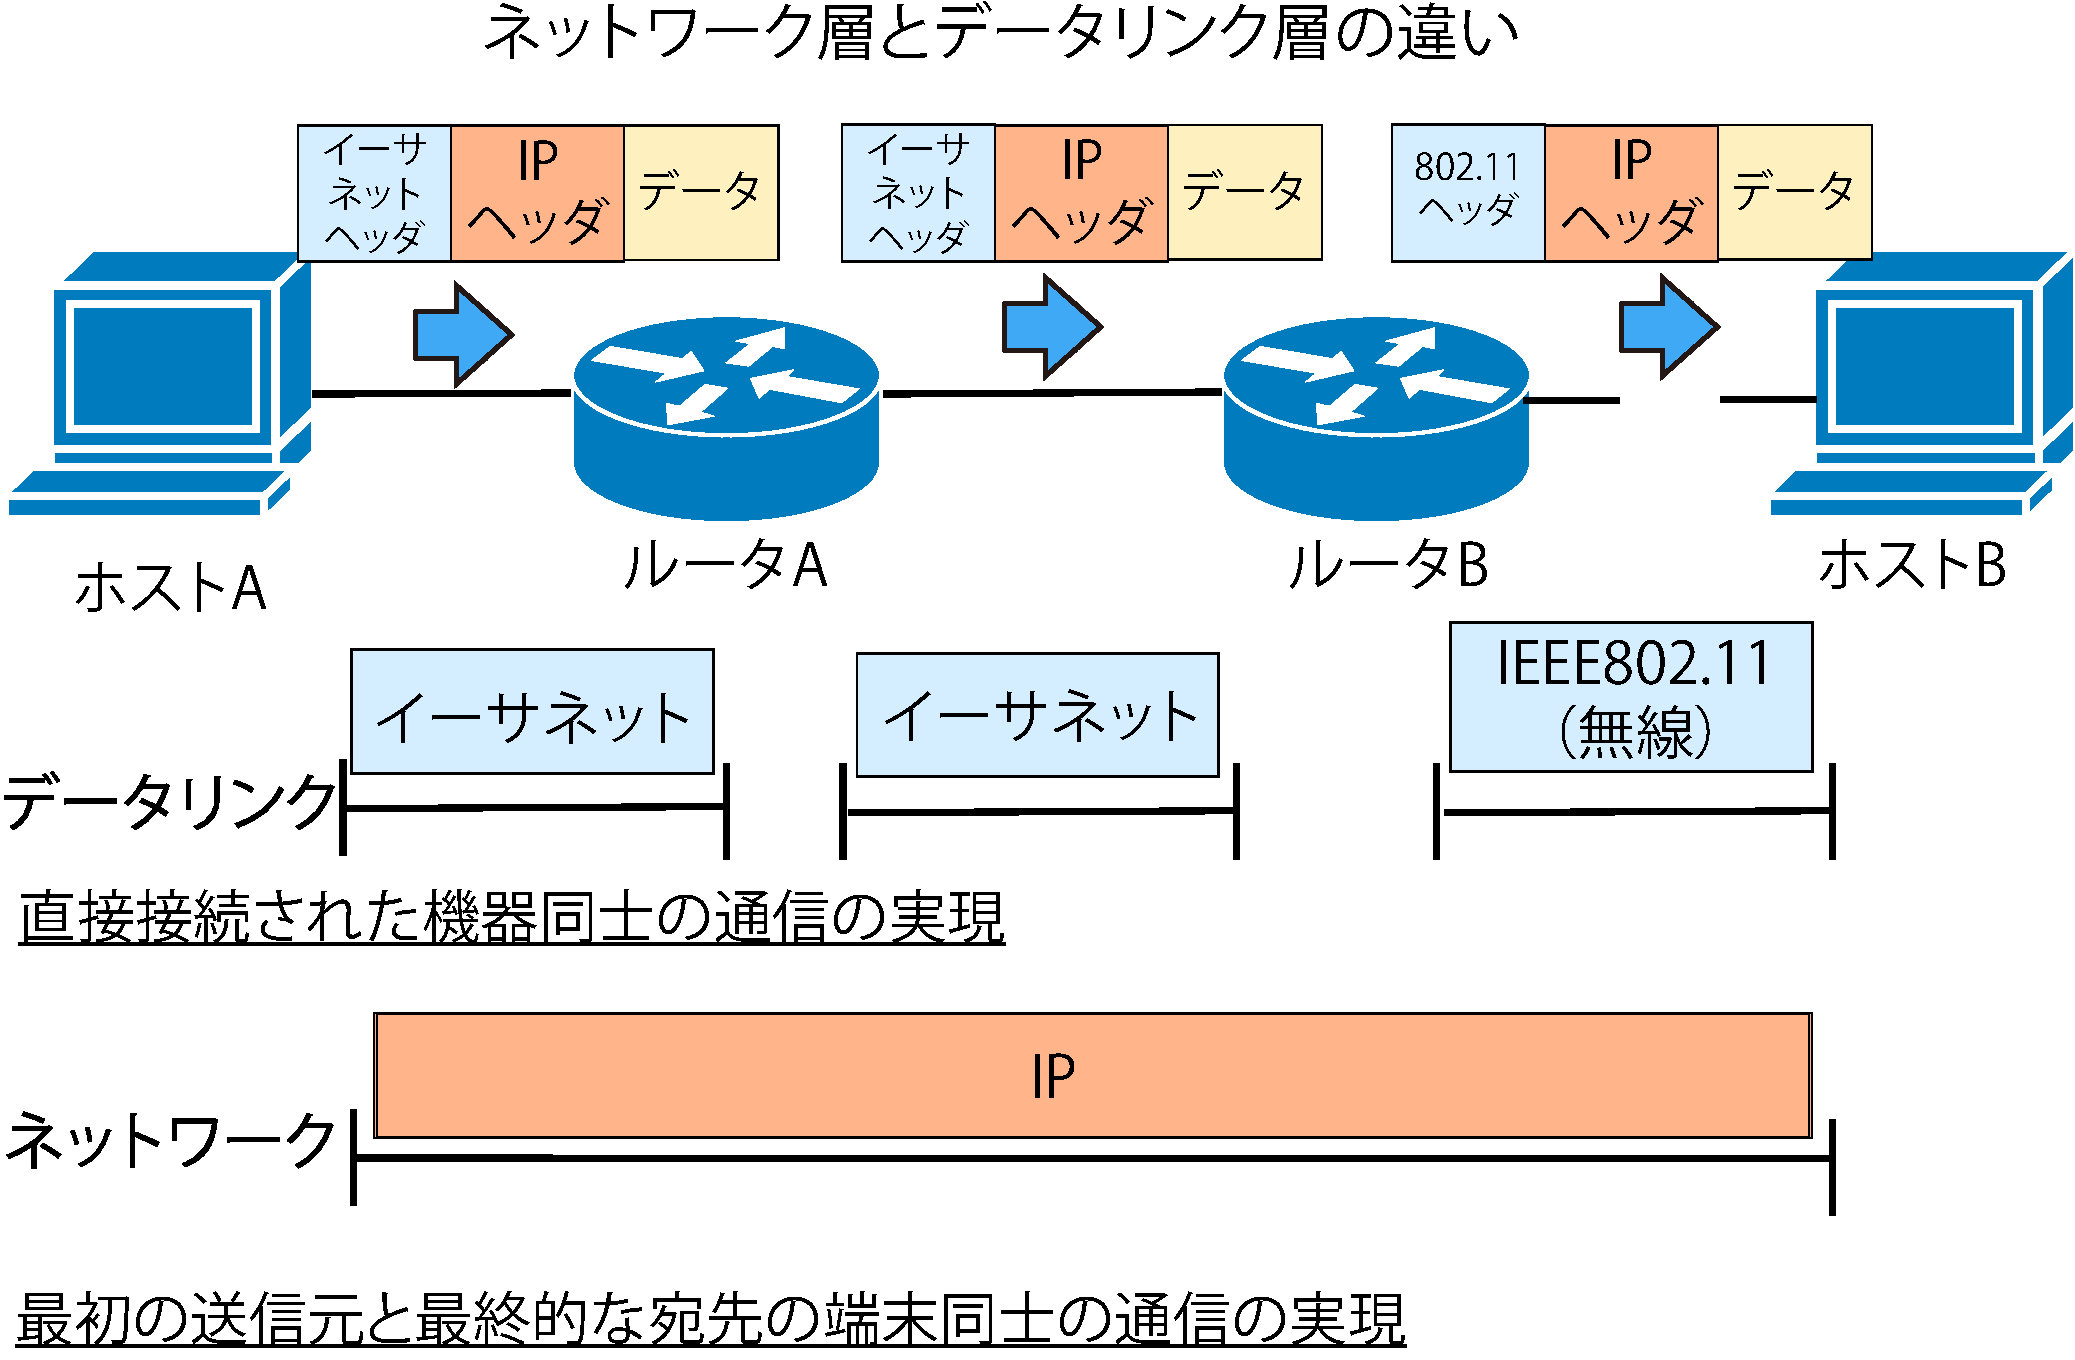
\includegraphics[clip,width=160mm]{figures/data_net.pdf}
\caption[データリンク層とネットワーク層の違い]{データリンク層とネットワーク層の違い\linebreak}
\label{fig:data_net}
\end{figure}

また,ネットワーク層の通信はIPというプロトコルによって宛先をIPアドレスで宛先を識別し,データリンク層は機器が固有に持つMACアドレスで宛先を識別している.
\clearpage
\subsubsection{IPアドレス}
IPアドレスとは,ネットワーク層のプロトコルであるIPで使用するアドレスであり,ネットワークに接続されているすべてのホストの中から通信を行う相手を識別する.
TCP/IPで通信するすべての機器には必ずIPアドレスを設定する必要がある.
IPはバージョンによる規格の違いが存在し,現在のネットワークでは「IPv4」と「IPv6」が主に利用されている.
バージョンによってIPアドレスの長さや表記が異なる.
「IPv4」と「IPv6」の違いの例を表\ref{table:ipv}に表す.\\

\begin{table}[hbtp]
  \caption{「IPv4」と「IPv6」の主な違い}
  \label{table:ipv}
  \centering
  \begin{tabular}{|l|c|c|}
    \hline
    名称  & 表記方法  &  例  \\
    \hline
    \hline 
    IPv4  & 32ビットを8ビットごとに区切り,10進数  & 192.168.130.10 \\
    \hline
    IPv6  & 128ビットを16ビットごとに区切り,16進数 & FEDC:BA98:7896:3210:BA76:AAB4:7654:23B0 \\
    \hline
  \end{tabular}
\end{table}
アドレスの長さや表記以外にも,ヘッダの構造や拡張機能の有無などの違いがある.
\subsubsection{MACアドレス}
MACアドレスとは,直接接続された機器を識別するためのアドレスである.IEEE802.3で規格化されたMACアドレスがイーサネット,無線LAN,Bluetoothなどで利用される.
IEEE(Institute of Electrical and Electronics Engineers)は,電気・情報工学分野の技術標準化機関であり,IEEE802委員会がLANに関連する規格を定めている.
MACアドレスは,一般的にコンピュータやルータなどのネットワークインタフェースカードに製造時に割り振られている.
全世界でMACアドレスが重複しないようになっており,意図的に変更したり仮想環境で設定しない限りは同じMACアドレスは存在しないため,直接接続された機器を識別することができる.
48ビットを8ビットごとに6つのオクテットに区切り,16進数で表現される.
\clearpage

\subsection{イーサネット}
\subsubsection{概要}
イーサネット(Ethernet)とは,IEEE802.3で規格された通信規格であり,有線LANを構成するために利用される.
他のLANを構成するための通信規格に比べて,制御の仕組みが単純であったため安価なネットワークインタフェースカードが作られ普及した.
イーサネットは,OSI参照モデルのデータリンク層と物理層に相当する通信規格である.

\subsubsection{イーサネットフレーム}
イーサネットフレームとは,イーサネットの通信を行う際に使用するデータのフォーマットのことである.
図\ref{fig:ether}にデータリンクを流れるパケットとイーサネットフレームの概略図を示す.

\begin{figure}[h]
\centering
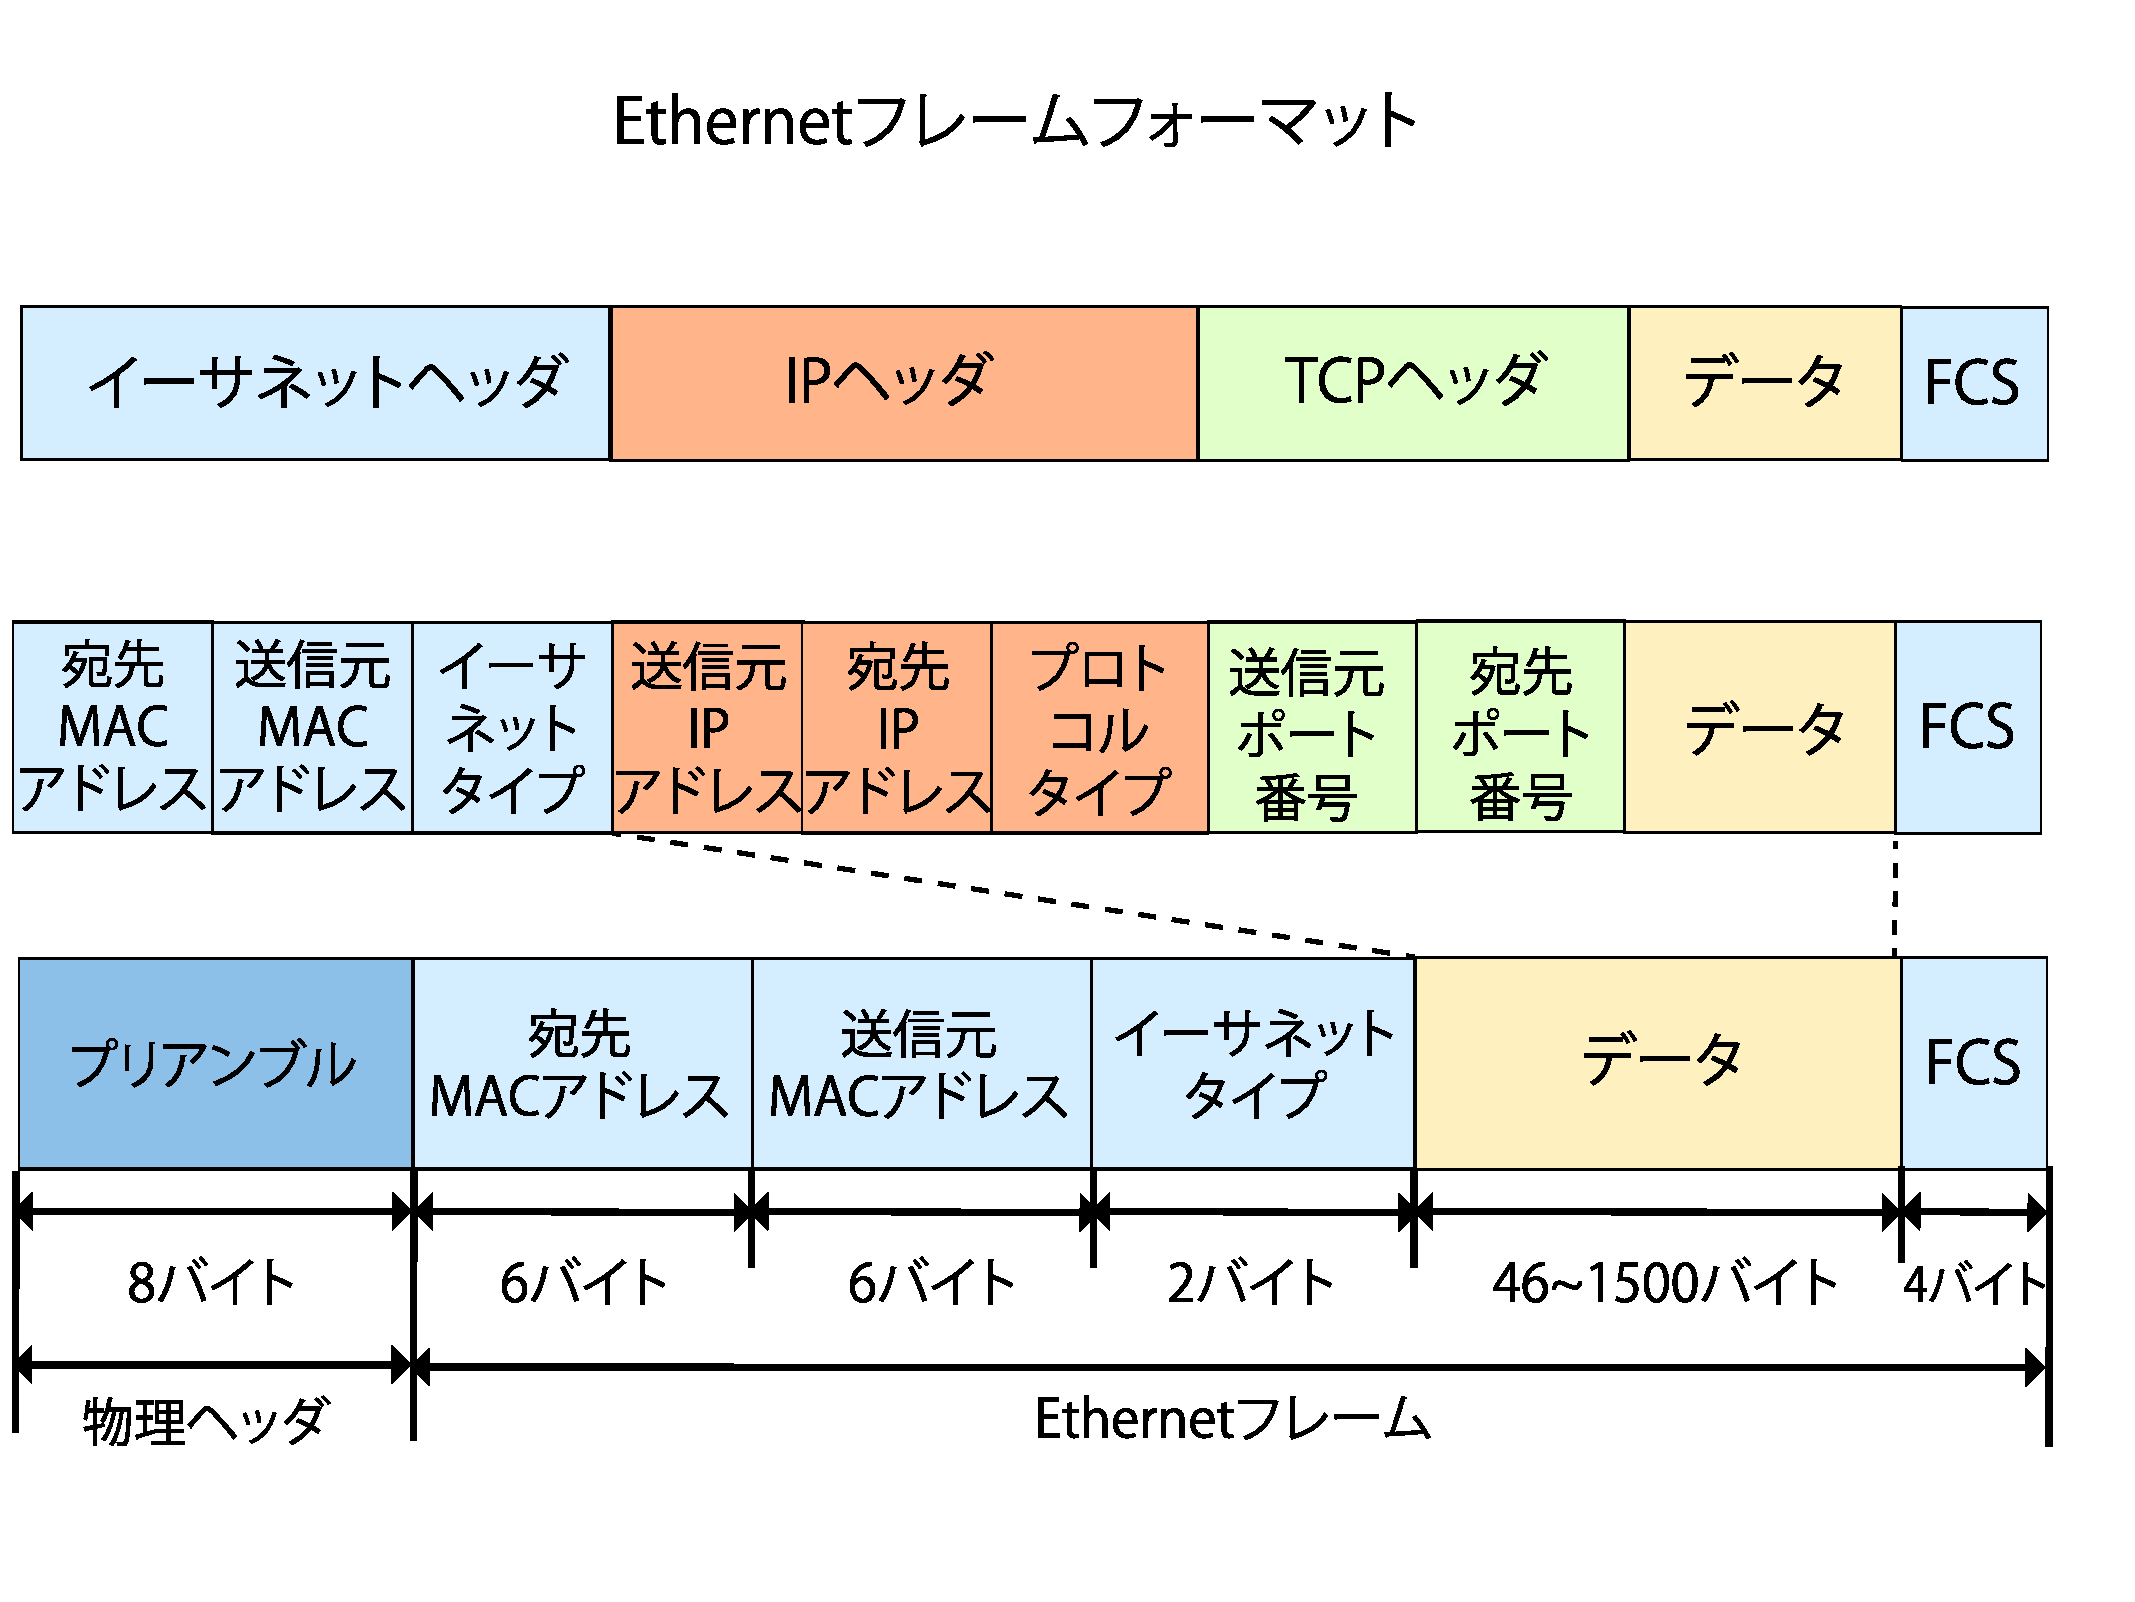
\includegraphics[clip,width=140mm]{figures/ethernet.pdf}
\caption[データリンクを流れるパケットとイーサネットフレームの概略図]{データリンクを流れるパケットとイーサネットフレームの概略図\linebreak}
\label{fig:ether}
\end{figure}

イーサネットフレームの各フィールドの説明を表に表す.
\\
\begin{table}[hbtp]
  \caption{イーサネットフレーム}
  \label{table:ipv}
  \centering
  \begin{tabular}{|l|c|}
    \hline
    フィールド名称  & フィールドの説明  \\
    \hline
    \hline 
    プリアンブル  & フレームの始まりを示すビット列 \\
    \hline 
    宛先MACアドレス  & 受信側のMACアドレス \\
    \hline 
    送信元MACアドレス  &  送信元のMACアドレス\\
    \hline 
    イーサネットタイプ  & データのプロトコルを識別する \\
    \hline 
    データ  & データリンク層より上位層のヘッダやデータ \\
    \hline 
    FCS  & 受信したフレームの破損を確認する \\
    \hline
  \end{tabular}
\end{table}

\clearpage

\section{開発する教材のコンセプト}%<5章>
a
\subsection{学習目的}
\subsection{教材の利用環境}
\subsection{教材の学習内容}
\subsection{教材の画面設計}

\clearpage

\section{教材の画面構成}%<6章>
\subsection{概要}

\begin{figure}[h]
\begin{center}
 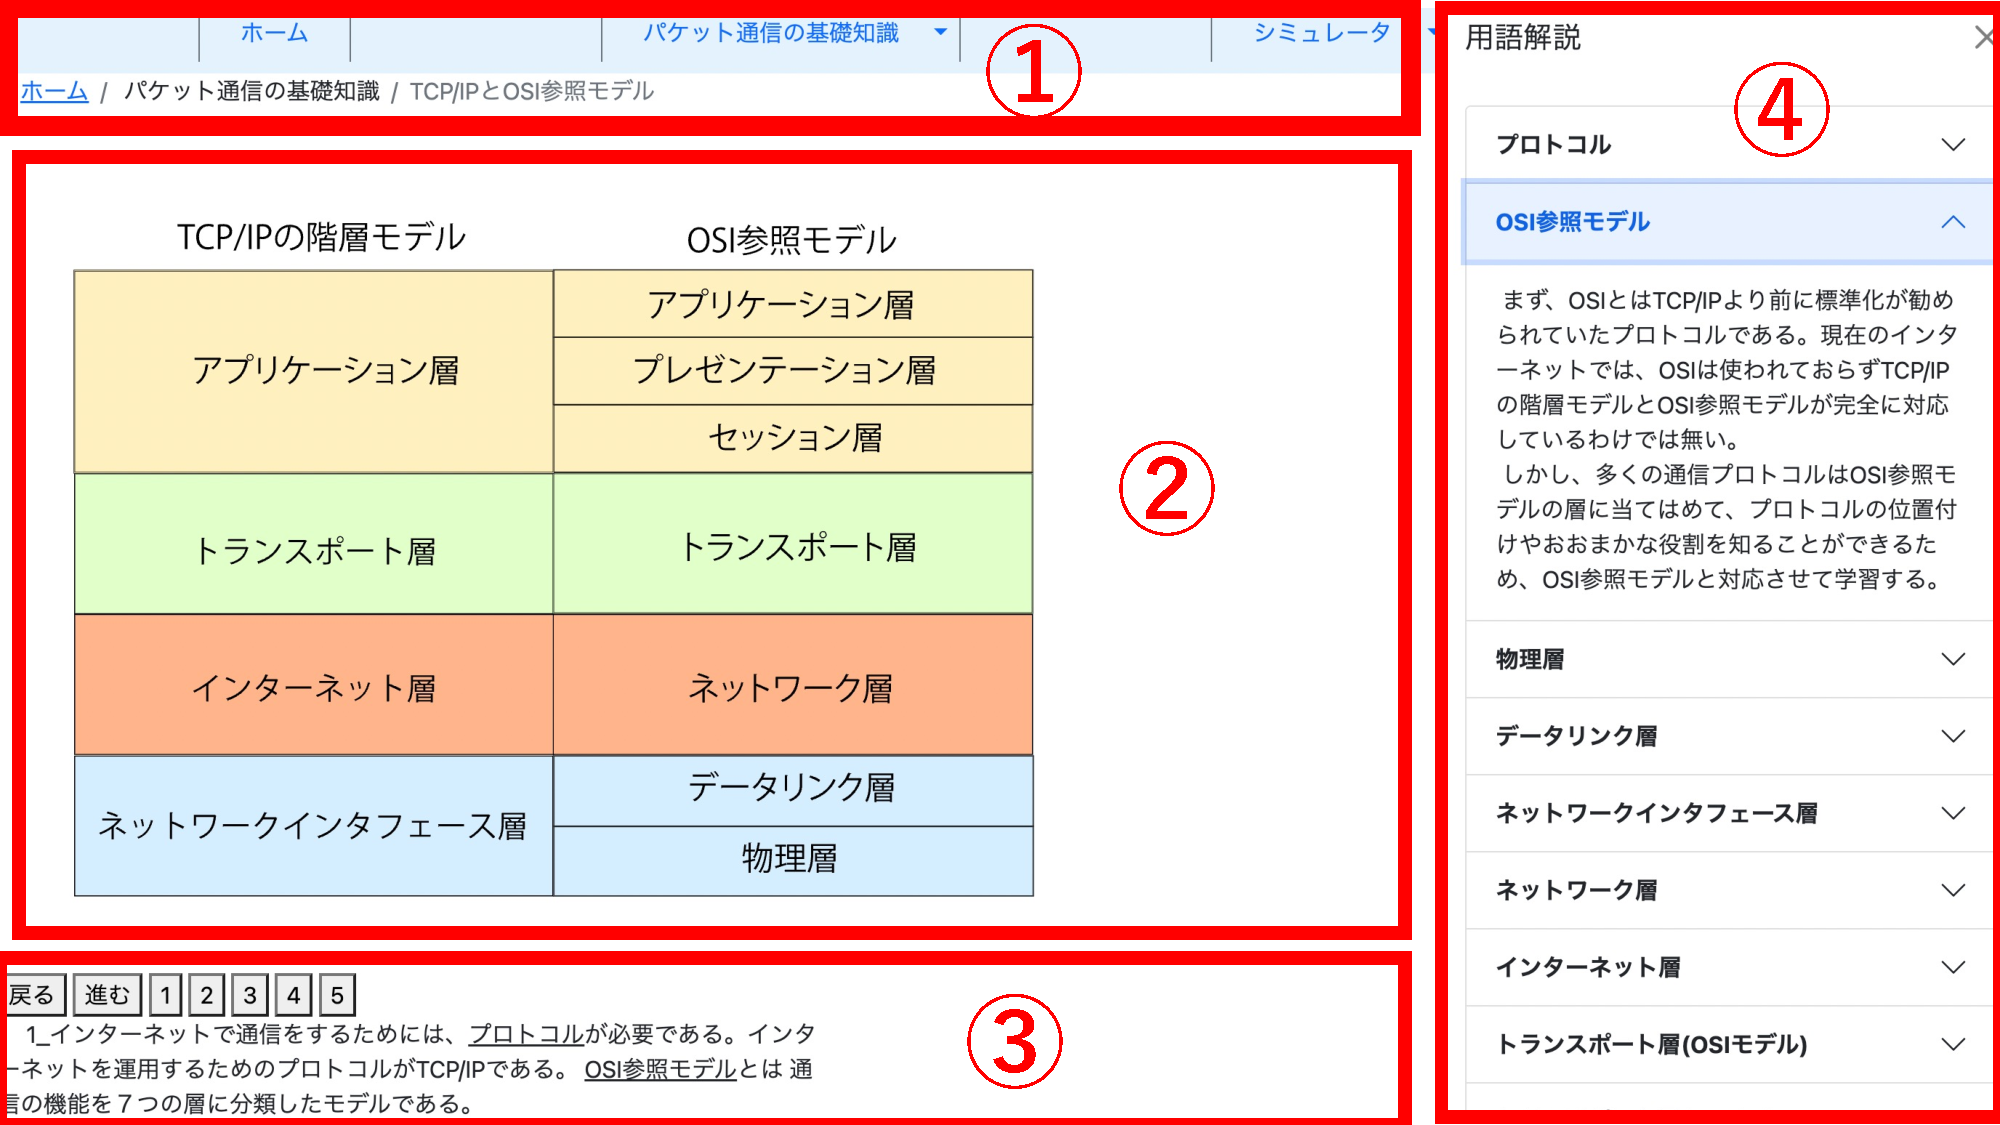
\includegraphics[clip,width=150mm]{figures/gamen.pdf}
\end{center}
 \caption{Web教材の学習画面1}
 \label{fig:画面}
\end{figure}

\subsection{ナビゲーション部}
\subsection{メイン表示部}
\subsection{解説表示部}
\subsection{用語解説部}
\subsection{シミュレータ設定部}
\begin{figure}[h]
\begin{center}
 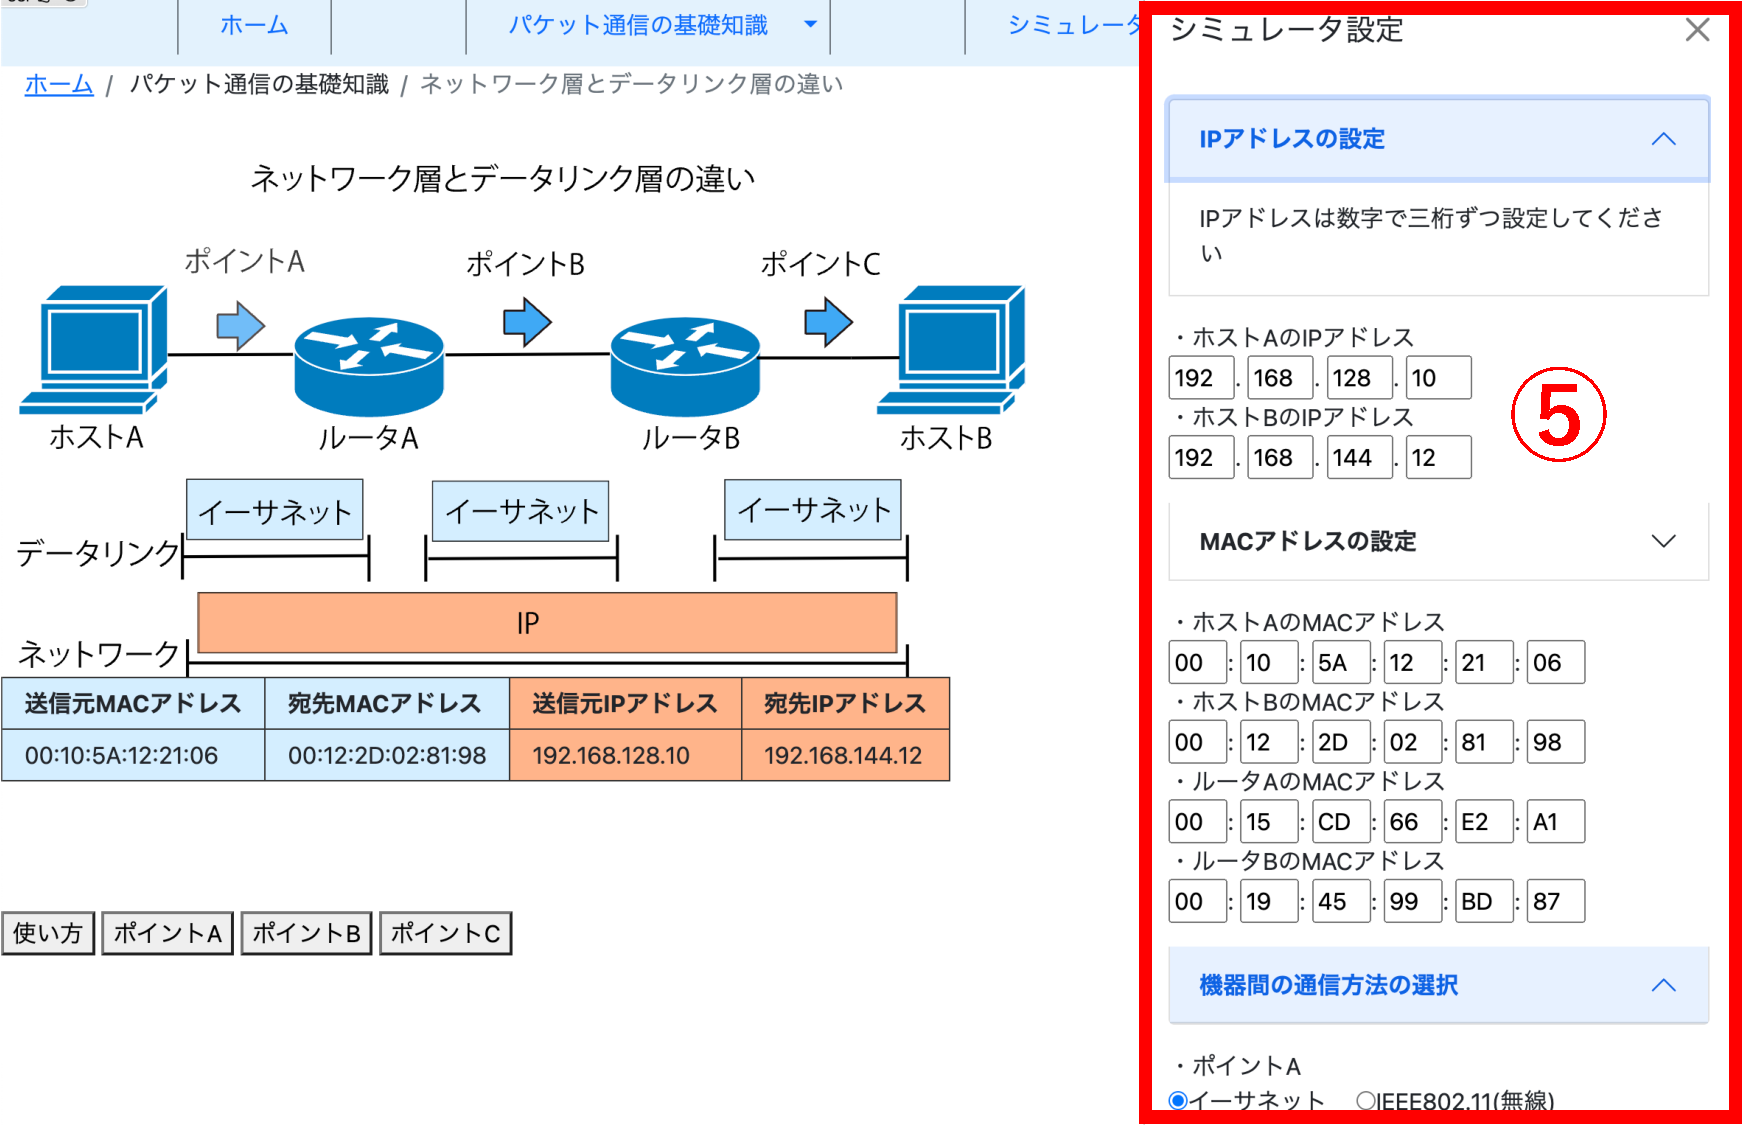
\includegraphics[clip,width=150mm]{figures/gamen2.pdf}
\end{center}
 \caption{Web教材の学習画面2}
 \label{fig:画面2}
\end{figure}
\clearpage

\section{教材の実装}%<7章>
a
\subsection{概要}
\subsection{開発に利用した言語}
\subsubsection{HTML}
HTMLとは,Hyper text Markup Languageの略称であり,ウェブページを作成するために開発された言語である.
\subsubsection{CSS}
\subsubsection{JavaScript}

\subsection{開発に利用したフレームワーク・ライブラリ}
\subsubsection{Bootstrap}
あ

\clearpage

\section{結言}%<8章>
a
%本研究では,ネットワーク通信の基礎を学習する講義形式の授業を補助するWeb教材を開発した.今後このような,生徒や学生が自分で操作し学習できるWeb教材が普及し,講義形式の授業で学習内容を深く理解できるようになることを期待している.
\clearpage

\section{謝辞}%<9章>
本研究の遂行及び本論文の作成にあたり,須田研究室の仲間に多くの手助けを頂きました,深く感謝の意を表します.そして,本論文の作成にあたり多大なる御指導及び御助言を頂きました,須田宇宙准教授に深く感謝の意を表します.
\clearpage

\begin{thebibliography}{99}
%2章
\bibitem{dx_kadai} 総務省: ``令和4年度版 情報通信白書 データ集(第3章第8節)'', 31,
\url{https://www.soumu.go.jp/johotsusintokei/whitepaper/ja/r04/html/nf308000.html#n3802030}, 2022/12/25参照

\bibitem{dx_gaiyou} 経済産業省: ``デジタルガバナンス・コード2.0'', \url{https://www.meti.go.jp/policy/it_policy/investment/dgc/dgc2.pdf}, 2022/12/25参照

%3章
\bibitem{kyoiku_gaiyou} 文部科学省: `` 「教育の情報化に関する手引」(案)第4章 情報教育'', \url{https://www.mext.go.jp/b_menu/shingi/chousa/shotou/056/gijigaiyou/attach/1259396.htm}, 2022/12/27参照

\bibitem{syogaku_pro} 文部科学省: `` 小学校プログラミング教育の手引(第三版)'', \url{https://www.mext.go.jp/content/20200218-mxt_jogai02-100003171_002.pdf}, 2022/12/27参照

\bibitem{syogaku_jirei} 文部科学省: `` 実施事例A一覧 | 未来の学びコンソーシアム '', \url{https://miraino-manabi.mext.go.jp/example/a}, 2023/01/03参照

\bibitem{tyugaku_29sidou} 文部科学省: `` 中学校学習指導要領(平成 29 年告示) - 文部科学省 '', \url{https://www.mext.go.jp/component/a_menu/education/micro_detail/__icsFiles/afieldfile/2018/05/07/1384661_5_4.pdf}, 2023/01/09参照

\bibitem{tyugaku_kyo1} 開隆堂出版株式会社: `` ネットワークを利用した双方向性のあるコンテンツのプログラミング 令和3年度用内容解説資料'',p2, \url{http://www.kairyudo.co.jp/contents/02_chu/gijutsu/r3/r3gi-souhoukou.pdf}, 2023/01/09参照

\bibitem{tyugaku_kyo2} 教育図書: `` 令和3年度用技術分野教科書パンフレット・誌面サンプル'',p8, \url{https://www.kyoiku-tosho.co.jp/b_data/2020/g702_naiyoukaisetsu/index.html}, 2023/01/09参照

\bibitem{tyugaku_kyo3} 東京書籍: `` 新しい技術・家庭 技術分野(中学校) 内容解説パンフレット '',p10, \url{https://ten.tokyo-shoseki.co.jp/text/chu/gijutsu/documents/gijutsu_naiyoukaisetsu.pdf}, 2023/01/09参照

\bibitem{tyugaku_kensyu} 文部科学省,: `` 事例1-2  D情報の技術 研修(D1) '',p8-9, \url{https://www.mext.go.jp/content/20210419-mxt_jogai01-000006333_003.pdf}, 2023/01/09参照

\bibitem{tyugaku_kensyu2} 文部科学省,: `` 事例2-2,2-3 D情報の技術 研修(D2)'',\url{https://www.mext.go.jp/content/20210419-mxt_jogai01-000006333_006.pdf}, 2023/01/09参照

\bibitem{tyugaku_jirei} 文部科学省,: `` 中学校技術・家庭科(技術分野)におけるプログラミング教育実践事例集②'',\url{https://www.mext.go.jp/content/20200403-mxt_jogai01-000006333_002.pdf}, 2023/01/09参照

\bibitem{koukou_sidou} 文部科学省: ``【情報編】高等学校学習指導要領(平成30年告示)解説'', \url{https://www.mext.go.jp/content/000166115.pdf}, 2023/1/10参照

\bibitem{koukou_kensyu} 文部科学省: ``【高等学校情報科「情報Ⅰ」教員研修用教材(本編)】第4章・巻末'', \url{https://www.mext.go.jp/content/20200722-mxt_jogai02-100013300_006.pdf}, 2023/1/10参照

\bibitem{koukou_jirei} 文部科学省: ``【実践事例】情報Ⅰ(3)(4)'', \url{https://www.mext.go.jp/content/000166207.pdf}, 2023/1/10参照

\bibitem{koukou_kon} 文部科学省: ``【授業・研修用コンテンツ 情報Ⅰ】学習動画 情報通信ネットワークとデータの活用'', \url{https://www.mext.go.jp/a_menu/shotou/zyouhou/detail/mext_01832.html}, 2023/1/10参照

\bibitem{koukou_anime} 数研出版 : ``数研出版 | 高等学校 情報Ⅰ | パケット通信'', \url{https://cds.chart.co.jp/books/ekq2rpke5d/lessons/097}, 2023/1/11参照

\bibitem{koukou_qr} 日本文教出版 : ``教科書QRコンテンツ|情報Ⅰ|高等学校 情報|日本文教出版'', \url{https://www.nichibun-g.co.jp/textbooks/joho/2022_joho01_1/qr/}, 2023/1/11参照

\bibitem{koukou_kyokasyo} 実教出版 : ``令和5年度用 情報パンフレット'', \url{https://www.jikkyo.co.jp/material/dbook/jouhou_r05/?pNo=1}, 2023/1/11参照

\bibitem{koukou_douga1} 情報処理学会 : ``IPSJ MOOC(登録不要、無料) - ご案内'', \url{https://sites.google.com/a.ipsj.or.jp/mooc/about?authuser=0}, 2023/1/11参照

\bibitem{koukou_douga2} 情報処理学会 : ``IPSJ MOOC(登録不要、無料) - 情報通信ネットワークの仕組みと役割'', \url{https://sites.google.com/a.ipsj.or.jp/mooc/list/C4-2?authuser=0}, 2023/1/11参照

\bibitem{koukou_dejikyo} 文部科学省: ``デジタル教科書に関する制度・現状について - 文部科学省'', \url{https://www.mext.go.jp/content/20200710-mxt_kyokasyo-000008653_03.pdf}, 2023/1/25参照
%https://ipsj.ixsq.nii.ac.jp/ej/?action=repository_uri&item_id=195372&file_id=1&file_no=1
\end{thebibliography}

\end{document}
